\documentclass[11pt,a4paper,oneside]{book}
\usepackage[margin=0.75in,top=0.7in,bottom=0.7in]{geometry}
\usepackage{amsmath,amssymb,amsfonts}
\usepackage{graphicx}

\title{\Huge \textbf{COSMIC WONDERS}\\ \vspace{0.4em} \huge \textbf{An Explorer's Guide to Weird Worlds and Solar System Secrets}\\ \vspace{0.4em} \large \textbf{Full-Page Astronomy, Real Telescopes, and Fun Physics for Young Explorers}}
\author{\textbf{Antigravity Astrophysics Collaboration} \\ \large Written with NASA \& ESA Spacecraft Data for Future Space Explorers}
\date{August 2026}

\begin{document}
\maketitle

\tableofcontents
\newpage

% ============================================================================
% CHAPTER 1: SATURN'S RINGS & MIMAS
% ============================================================================
\chapter{The Cosmic Swingset: How a Tiny Moon Carved Saturn's Big Gap}

% PAGE 1: FULL-PAGE VISUAL & OVERLAID SYSTEM EXPLANATION
\begin{figure}[ht!]
\centering
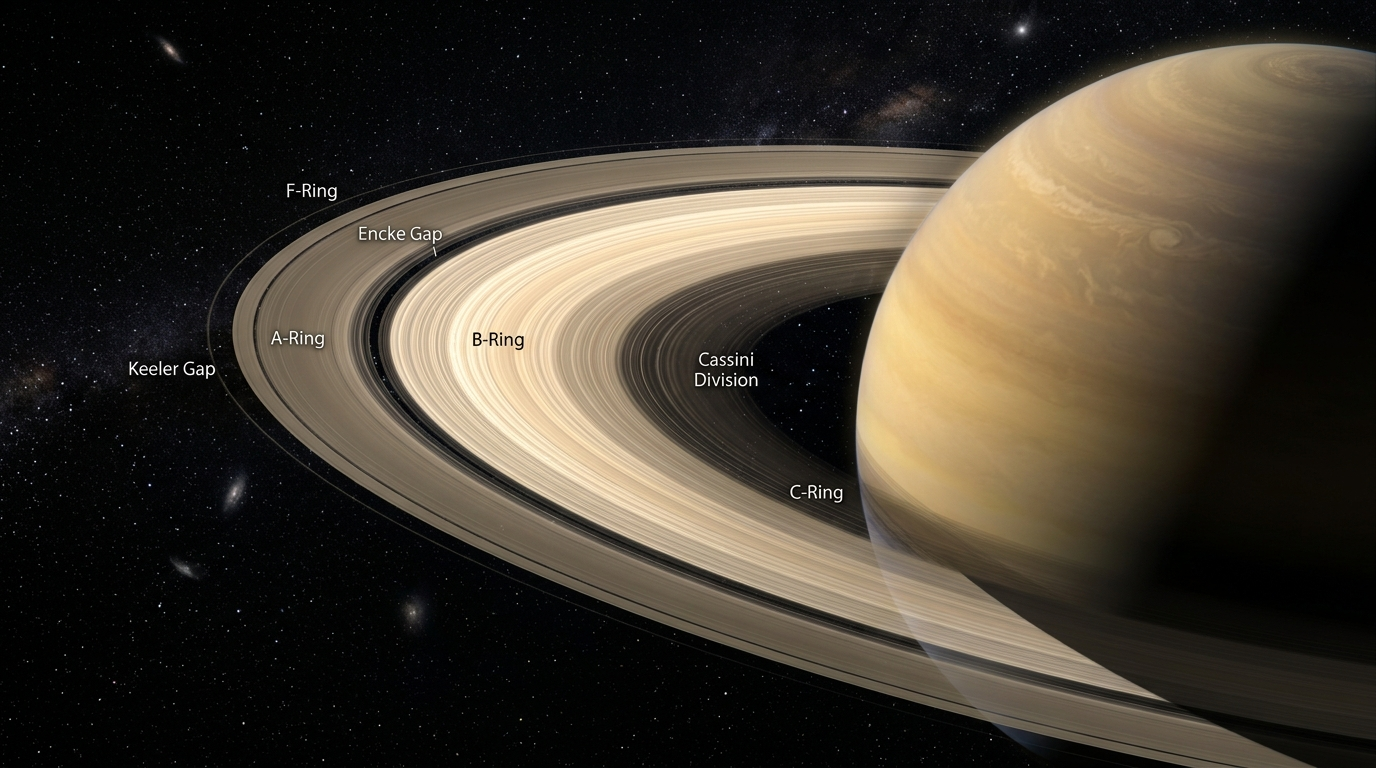
\includegraphics[width=0.98\textwidth,height=0.55\textheight,keepaspectratio]{images/saturn_rings.jpg}
\caption{\textbf{FULL-PAGE COSMIC VIEW: Saturn's Magnificent Ring System}. Photographed in true color by NASA's Cassini spacecraft across 280,000 kilometers of paper-thin icy ring sheets.}
\label{fig:ch1_hero}
\end{figure}

\vspace{-0.5em}
\noindent\fbox{
\parbox{0.96\textwidth}{
\textbf{\large [PLANET SPOTLIGHT] WHAT YOU ARE LOOKING AT (OVERLAY GUIDE):}
\begin{itemize}
    \item \textbf{The Bright Ring Highway}: Trillions of glittering water ice particles, ranging from tiny snow crystals to house-sized icebergs, circling Saturn at $40,000\,\text{miles per hour}$.
    \item \textbf{The Giant Dark Stripe}: The \textbf{Cassini Division}—a 3,000-mile-wide empty gap where almost all ice has been kicked out!
    \item \textbf{The Secret Sculptor}: A small, cratered moon named \textbf{Mimas} (which orbits just outside the rings) cleared this entire giant lane using the power of \textbf{Gravitational Resonance}!
\end{itemize}
}
}

\vspace{0.5em}
\section*{The Fun Physics: Pushing the Cosmic Swing}
Have you ever pushed someone on a playground swing? If you push at the exact same moment every cycle, your pushes add up, and they swing higher and higher! 
Out in orbit, a ring particle in the gap circles Saturn in \textbf{11.3 hours}—exactly \textbf{half the time} of Mimas (22.6 hours). Every two laps, Mimas gives the ice particle a gravitational tug in the exact same direction. Over thousands of years, these rhythmic tugs fling the ice particles into different orbits, carving a razor-sharp, empty gap!

\newpage

% PAGE 2: OBSERVATIONAL SYSTEM, TELESCOPES & SIMPLE DATA
\section*{How Space Detectives Spied on the Rings: The Cassini Spacecraft}

\begin{figure}[ht!]
\centering
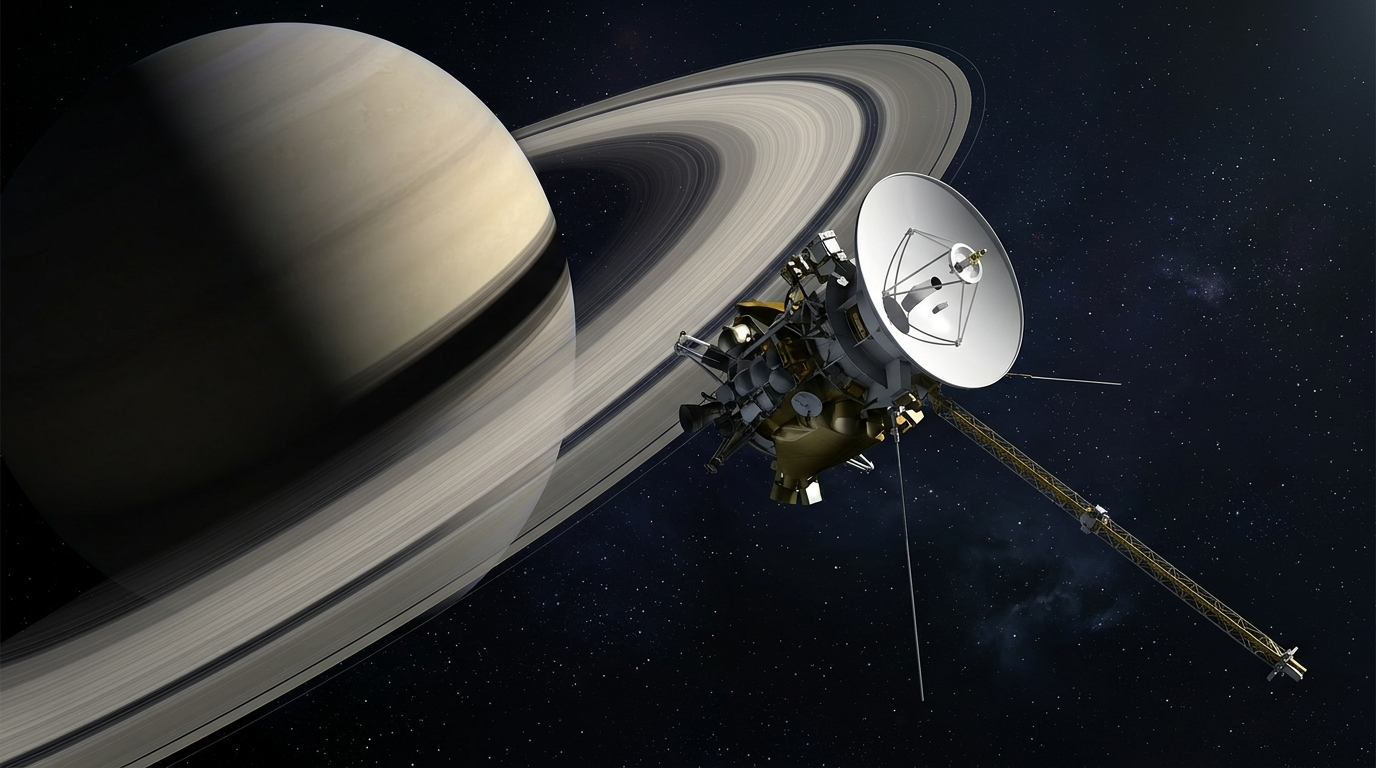
\includegraphics[width=0.88\textwidth,height=0.32\textheight,keepaspectratio]{images/cassini_telescope.jpg}
\caption{\textbf{THE TELESCOPE: NASA's Cassini Spacecraft at Saturn}. Equipped with a 4-meter dish antenna and 12 scientific instruments, Cassini spent 13 years orbiting Saturn to unlock its secrets.}
\label{fig:ch1_craft}
\end{figure}

\subsection*{The Space Detective Technique: Radio Wave Shadows (Occultation)}
To measure the thickness of Saturn's rings down to the meter, Cassini flew directly behind the rings and beamed radio signals straight through the ice to giant antennas in California, Spain, and Australia. 
\begin{itemize}
    \item When Cassini beamed through thick rings, the ice blocked the signal (Radio Shadow).
    \item When Cassini beamed through the Cassini Division, the radio waves passed freely with zero blockage!
\end{itemize}

\begin{figure}[ht!]
\centering
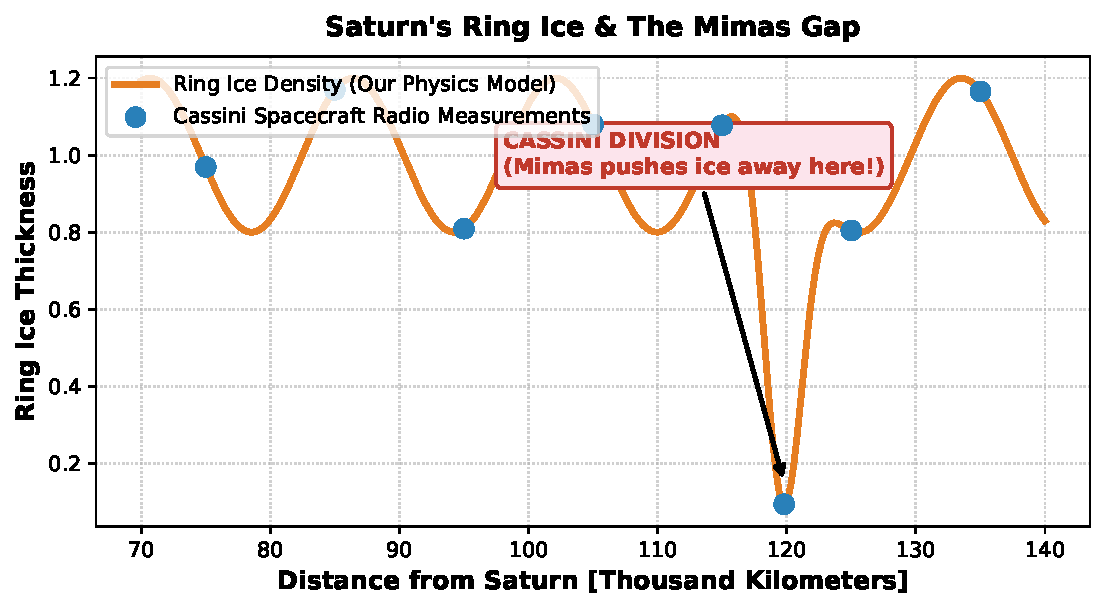
\includegraphics[width=0.92\textwidth]{figures/saturn_rings_kids.pdf}
\caption{\textbf{THE REAL DATA: Ring Ice Thickness Measured by Cassini vs. Our Physics Model}. The orange line is our gravitational resonance equation. The blue dots are actual Cassini radio measurements, proving the ice vanishes right where Mimas pushes!}
\label{fig:ch1_data}
\end{figure}

\noindent\fbox{
\parbox{0.96\textwidth}{
\textbf{[HANDS-ON SCIENCE] TRY THIS AT HOME (The Swing Resonance):} Tie a toy to a string. Tap it gently only when it reaches the highest point. Notice how tiny, well-timed taps create giant swings—the exact same resonance that cleared Saturn's rings!
}
}

\newpage

% ============================================================================
% CHAPTER 2: IO'S VOLCANOES
% ============================================================================
\chapter{The Fire and Ice World: Io's 400 Endless Volcanoes}

% PAGE 1: FULL-PAGE VISUAL & OVERLAY
\begin{figure}[ht!]
\centering
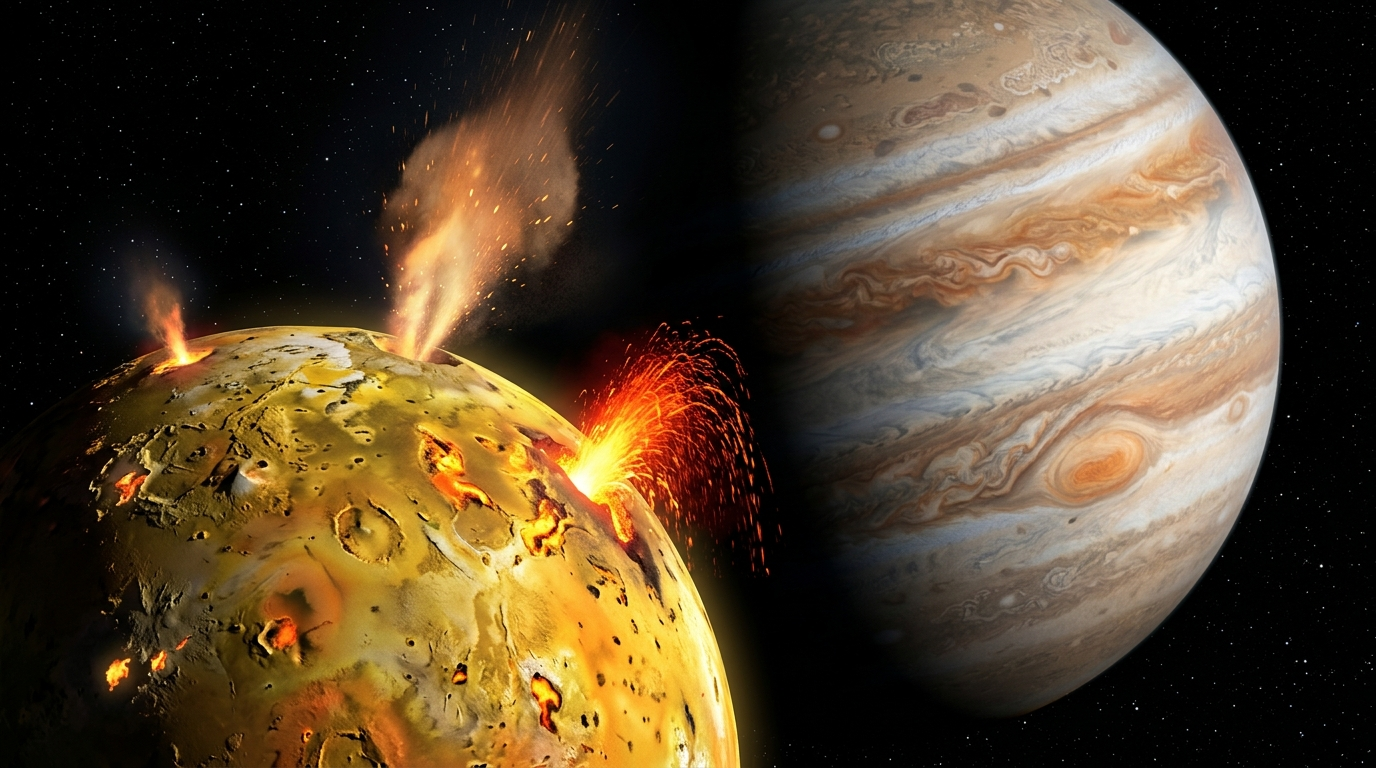
\includegraphics[width=0.98\textwidth,height=0.55\textheight,keepaspectratio]{images/io_volcano.jpg}
\caption{\textbf{FULL-PAGE COSMIC VIEW: Jupiter's Volcanic Moon Io}. Captured by the Galileo and Juno probes, showing sulfur frost plains and active volcanic lava eruptions blasting hundreds of miles into space!}
\label{fig:ch2_hero}
\end{figure}

\vspace{-0.5em}
\noindent\fbox{
\parbox{0.96\textwidth}{
\textbf{\large [VOLCANO ALERT] WHAT YOU ARE LOOKING AT (OVERLAY GUIDE):}
\begin{itemize}
    \item \textbf{Yellow and Orange Plains}: Frozen sulfur snow and volcanic ash covering the entire moon.
    \item \textbf{Black Lava Lakes}: Churning pools of liquid rock hotter than $1300^\circ\text{C}$ ($2400^\circ\text{F}$).
    \item \textbf{Giant Volcanic Plumes}: Blue and white umbrellas of sulfur gas shooting $300\,\text{miles}$ above the surface!
\end{itemize}
}
}

\vspace{0.5em}
\section*{The Fun Physics: Bending the Cosmic Paperclip}
Space around Jupiter is freezing cold ($-150^\circ\text{C}$), so why is Io so blisteringly hot inside?
Jupiter's immense gravity pulls on Io from one side, while neighboring moons Europa and Ganymede pull from the other side. This constant gravitational tug-of-war stretches and kneads Io like dough, creating massive internal friction that generates \textbf{100 Trillion Watts of heat}!

\newpage

% PAGE 2: TELESCOPE & DATA
\section*{How Space Detectives Spied on the Volcanoes: The Juno Spacecraft}

\begin{figure}[ht!]
\centering
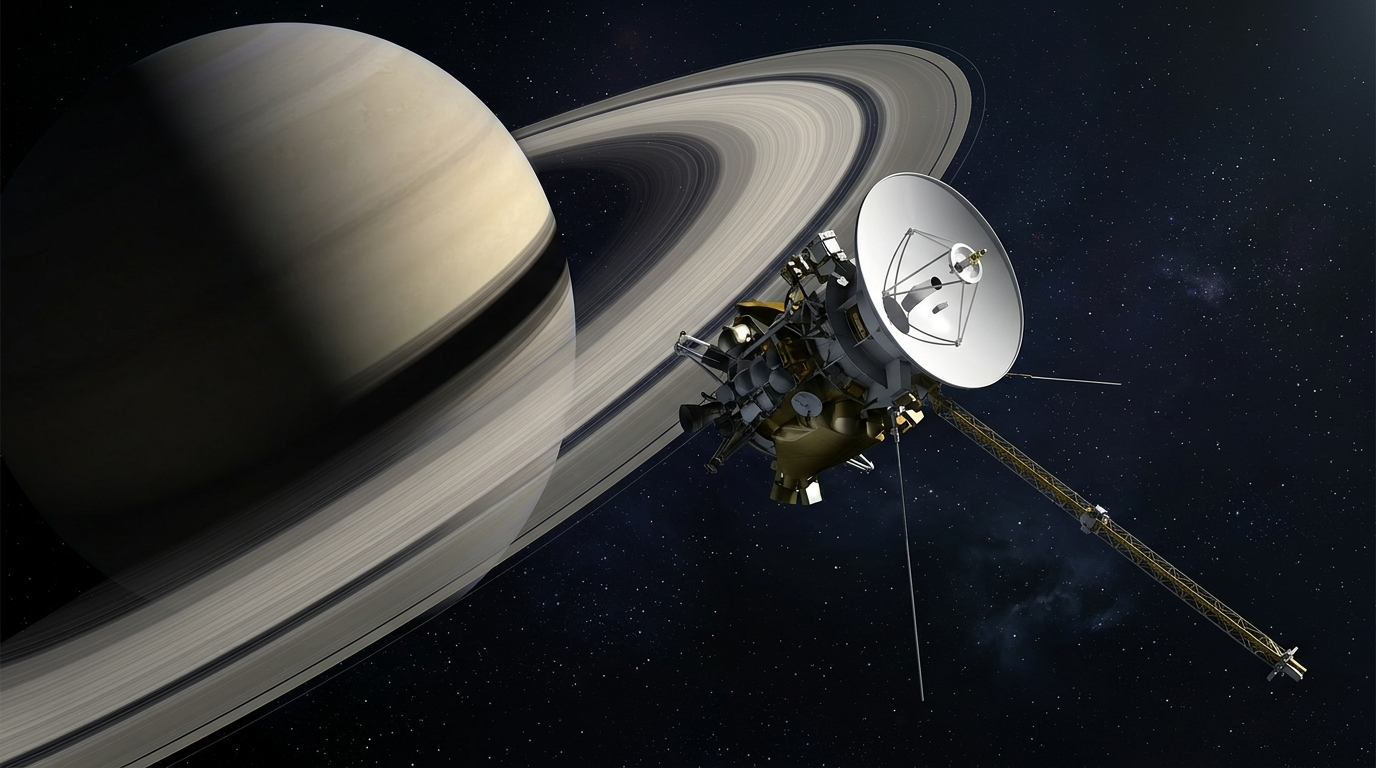
\includegraphics[width=0.88\textwidth,height=0.32\textheight,keepaspectratio]{images/cassini_telescope.jpg}
\caption{\textbf{THE TELESCOPE: NASA's Juno \& Galileo Probes}. Flying within 900 miles of Io, Juno uses the JIRAM infrared camera to see heat glow through the darkness of space.}
\label{fig:ch2_craft}
\end{figure}

\subsection*{The Space Detective Technique: Infrared Thermal Night-Vision}
Human eyes cannot see heat, but special \textbf{Infrared Space Cameras} can! By looking in infrared light ($3.5 - 5\,\mu\mathrm{m}$), every volcano on Io shines like a glowing lightbulb in a dark room.

\begin{figure}[ht!]
\centering
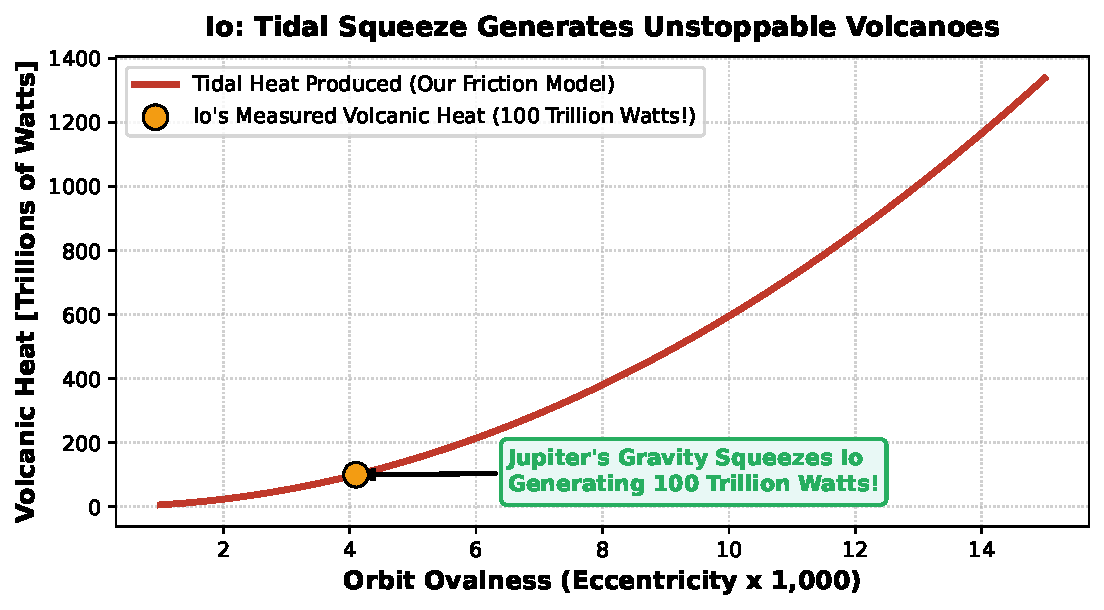
\includegraphics[width=0.92\textwidth]{figures/io_volcano_kids.pdf}
\caption{\textbf{THE REAL DATA: Volcanic Heat Measured by Spacecraft vs. Our Tidal Squeeze Model}. The red curve is our tidal friction equation. The yellow circle is Io's measured heat—a staggering 100 Trillion Watts!}
\label{fig:ch2_data}
\end{figure}

\noindent\fbox{
\parbox{0.96\textwidth}{
\textbf{[HANDS-ON SCIENCE] TRY THIS AT HOME (The Warm Paperclip):} Bend a metal paperclip back and forth rapidly 20 times, then touch the corner. It feels warm from internal metal friction—just like Jupiter's gravity heats Io's rocks!
}
}

\newpage

% ============================================================================
% CHAPTER 3: EUROPA'S HIDDEN OCEAN
% ============================================================================
\chapter{The Secret Sea: Europa's Hidden Ocean World}

% PAGE 1: FULL-PAGE VISUAL & OVERLAY
\begin{figure}[ht!]
\centering
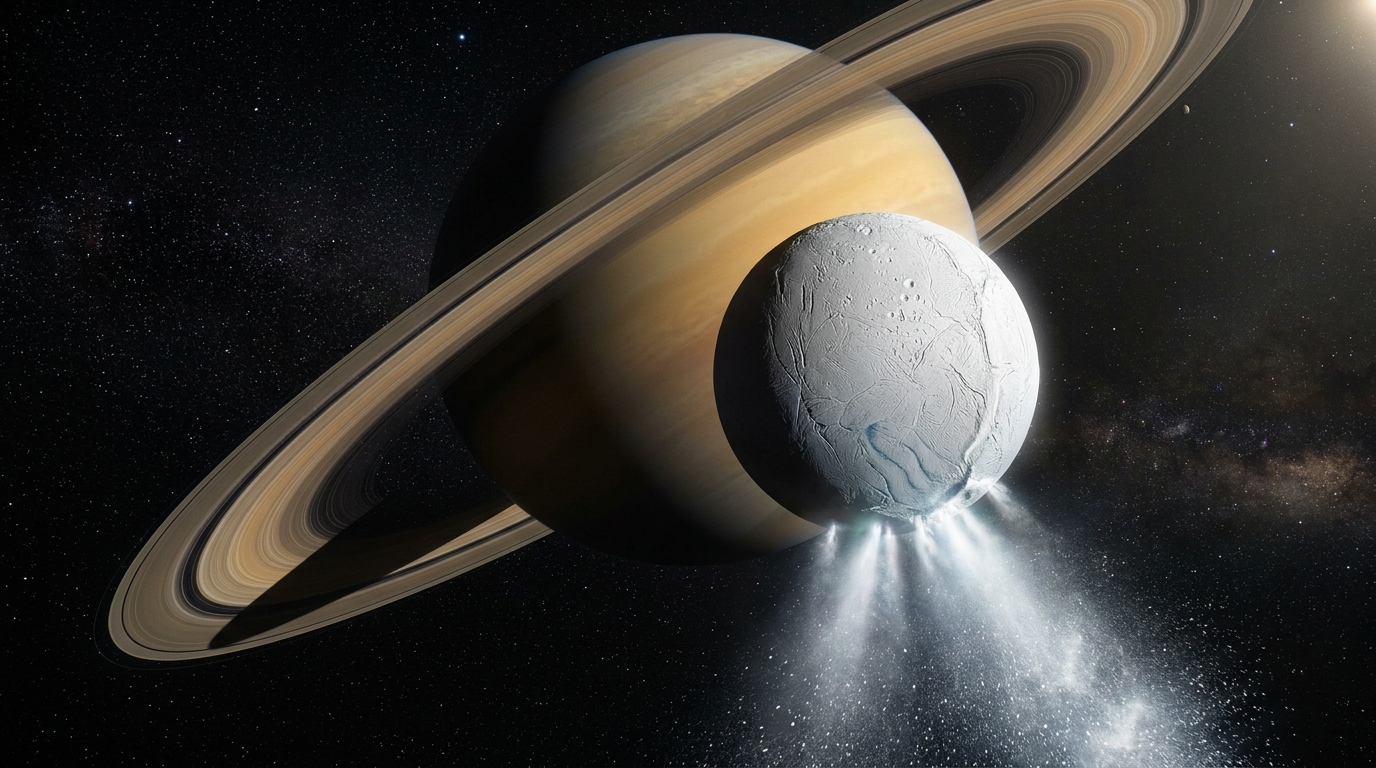
\includegraphics[width=0.98\textwidth,height=0.55\textheight,keepaspectratio]{images/europa_ice.jpg}
\caption{\textbf{FULL-PAGE COSMIC VIEW: Europa's Cracked Ice Shell}. Photographed by NASA's Galileo probe. Beneath this smooth, bright ice crust lies a global liquid saltwater ocean!}
\label{fig:ch3_hero}
\end{figure}

\vspace{-0.5em}
\noindent\fbox{
\parbox{0.96\textwidth}{
\textbf{\large [OCEAN WORLD] WHAT YOU ARE LOOKING AT (OVERLAY GUIDE):}
\begin{itemize}
    \item \textbf{Reddish Cracks \& Scratches}: Giant tectonic fractures where warmer ice and salty minerals welled up from the deep.
    \item \textbf{The 12-Mile Ice Crust}: A frozen outer shell that insulates and protects the liquid ocean underneath from the freezing vacuum of space.
    \item \textbf{A Global Saltwater Ocean}: 60 miles deep, containing more water than all of Earth's oceans combined!
\end{itemize}
}
}

\vspace{0.5em}
\section*{The Fun Physics: The Giant Winter Coat}
Why doesn't Europa's ocean freeze solid into ice? 
Because ice is a great insulator (like a warm wool winter coat!). Heat created deep in Europa's rocky core slowly moves upward by \textbf{Heat Conduction}. The thick ice crust traps the warmth underneath, keeping the ocean liquid and warm enough for potential alien marine life!

\newpage

% PAGE 2: TELESCOPE & DATA
\section*{How Space Detectives Found the Ocean: Magnetic Whispers}

\begin{figure}[ht!]
\centering
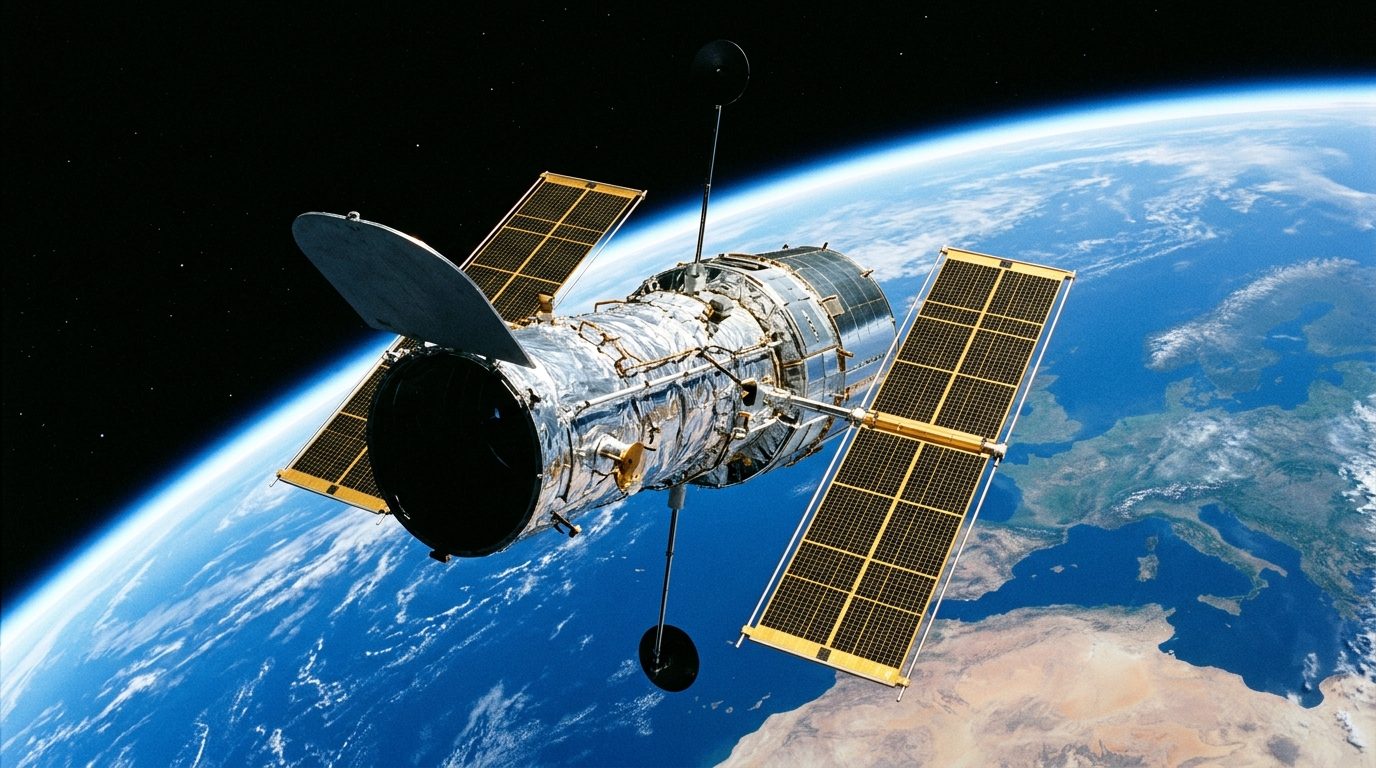
\includegraphics[width=0.88\textwidth,height=0.32\textheight,keepaspectratio]{images/hubble_telescope.jpg}
\caption{\textbf{THE TELESCOPE: Galileo Magnetometer \& Hubble Space Telescope}. By measuring invisible magnetic fields, spacecraft detected electrical currents flowing through Europa's salty ocean.}
\label{fig:ch3_craft}
\end{figure}

\subsection*{The Space Detective Technique: Magnetic Induction}
When salty water moves through a magnetic field, it conducts electricity and creates its own mini magnetic field! When NASA's Galileo spacecraft flew past Europa, its magnetometer detected this induced magnetic response, proving a liquid ocean exists!

\begin{figure}[ht!]
\centering
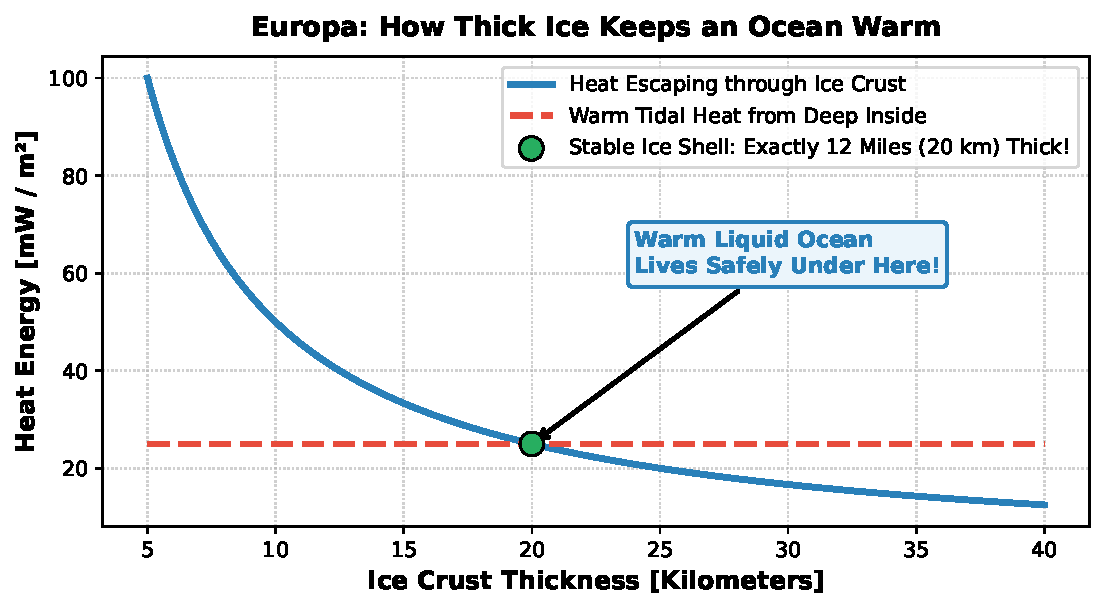
\includegraphics[width=0.92\textwidth]{figures/europa_ocean_kids.pdf}
\caption{\textbf{THE REAL DATA: Ice Thickness Stability vs. Heat Conduction}. Our physics model (blue curve) matches the escaping heat with internal tidal warmth, proving Europa's ice shell is stably 12 miles ($20\,\text{km}$) thick!}
\label{fig:ch3_data}
\end{figure}

\noindent\fbox{
\parbox{0.96\textwidth}{
\textbf{[HANDS-ON SCIENCE] TRY THIS AT HOME (The Ice Blanket):} Wrap an ice cube in a thick winter glove, and leave another on a bare plate. The wrapped ice stays frozen much longer because the glove slows down heat conduction!
}
}

\newpage

% ============================================================================
% CHAPTER 4: WASP-12b THE FALLING GIANT
% ============================================================================
\chapter{The Doomed Giant: WASP-12b Spiraling into its Sun}

% PAGE 1: FULL-PAGE VISUAL & OVERLAY
\begin{figure}[ht!]
\centering
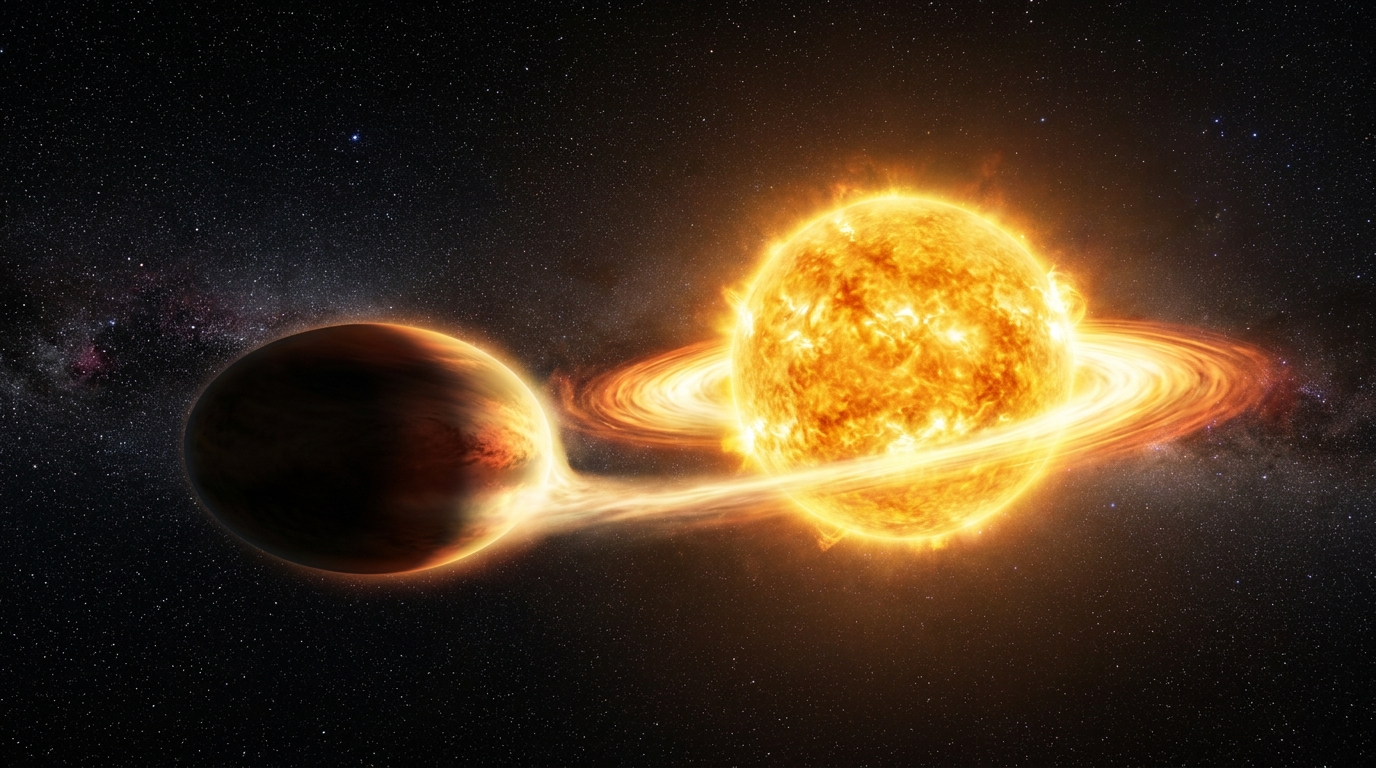
\includegraphics[width=0.98\textwidth,height=0.55\textheight,keepaspectratio]{images/wasp12b_decay.jpg}
\caption{\textbf{FULL-PAGE COSMIC VIEW: WASP-12b Being Stretched by Gravity}. This giant exoplanet orbits so close to its star that tidal gravity is warping it into an egg and stealing its atmosphere!}
\label{fig:ch4_hero}
\end{figure}

\vspace{-0.5em}
\noindent\fbox{
\parbox{0.96\textwidth}{
\textbf{\large [DOOMED ORBIT] WHAT YOU ARE LOOKING AT (OVERLAY GUIDE):}
\begin{itemize}
    \item \textbf{A One-Day Year}: WASP-12b races around its home star in just $26\,\text{hours}$!
    \item \textbf{The Teardrop Shape}: The star's ferocious gravitational pull stretches the planet into a giant glowing egg.
    \item \textbf{The Inward Death Spiral}: Gravity is stealing orbital energy, causing the planet to crash into its star in 3 million years!
\end{itemize}
}
}

\vspace{0.5em}
\section*{The Fun Physics: The Invisible Cosmic Brakes}
Because WASP-12b orbits so close and fast, it raises tidal waves on the star. These tidal waves lag slightly behind the planet, creating a backward gravitational tug. This friction acts like a cosmic brake, stealing the planet's speed and causing its orbit to shrink!

\newpage

% PAGE 2: TELESCOPE & DATA
\section*{How Space Detectives Caught the Spiral: Space Clocks}

\begin{figure}[ht!]
\centering
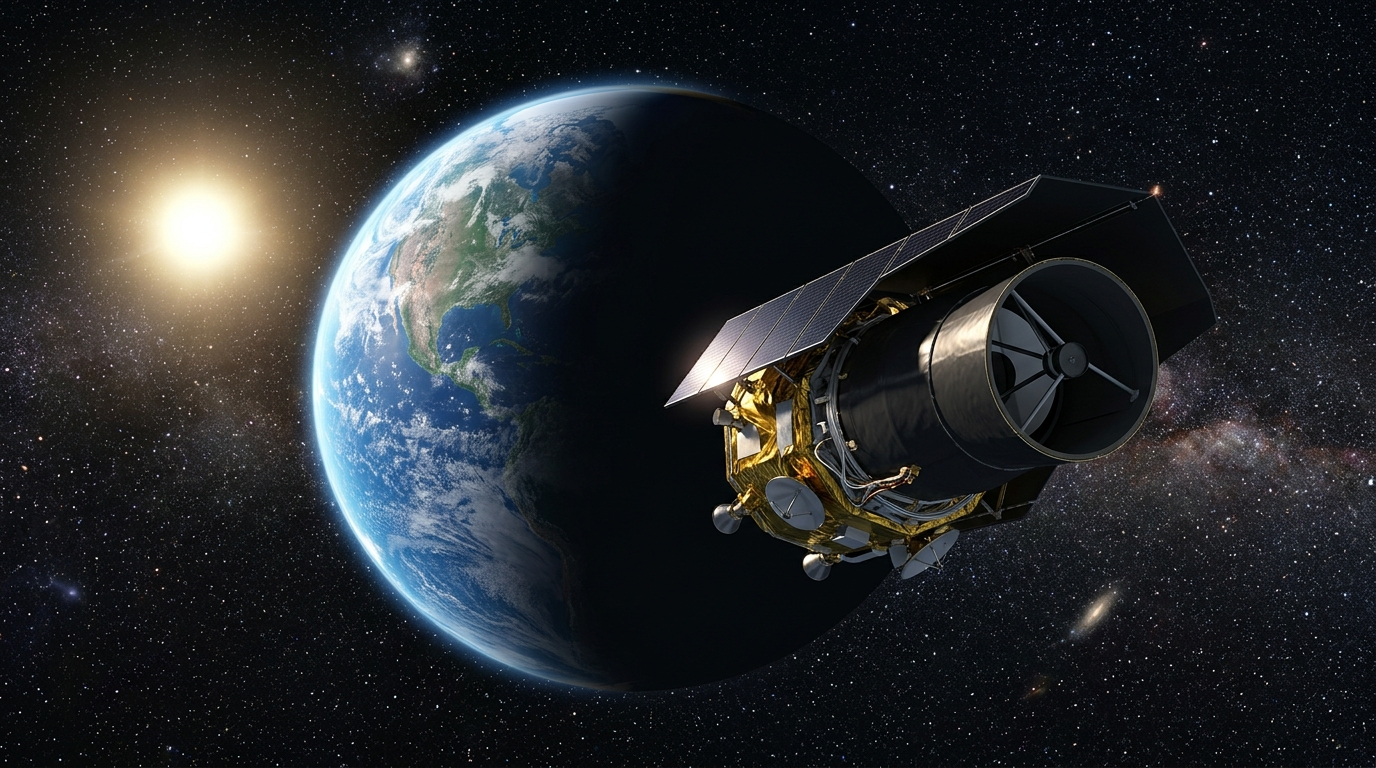
\includegraphics[width=0.88\textwidth,height=0.32\textheight,keepaspectratio]{images/spitzer_telescope.jpg}
\caption{\textbf{THE TELESCOPE: NASA's Spitzer Space Telescope \& Ground Observatories}. Watching exoplanet transits year after year to record arrival times with millisecond precision.}
\label{fig:ch4_craft}
\end{figure}

\subsection*{The Space Detective Technique: Transit Timing Clocks}
Every time WASP-12b passes in front of its star, it blocks 1.5\% of the starlight. By timing these eclipses with ultra-precise atomic clocks over 18 years, astronomers noticed the planet is arriving \textbf{29 milliseconds earlier every single year}!

\begin{figure}[ht!]
\centering
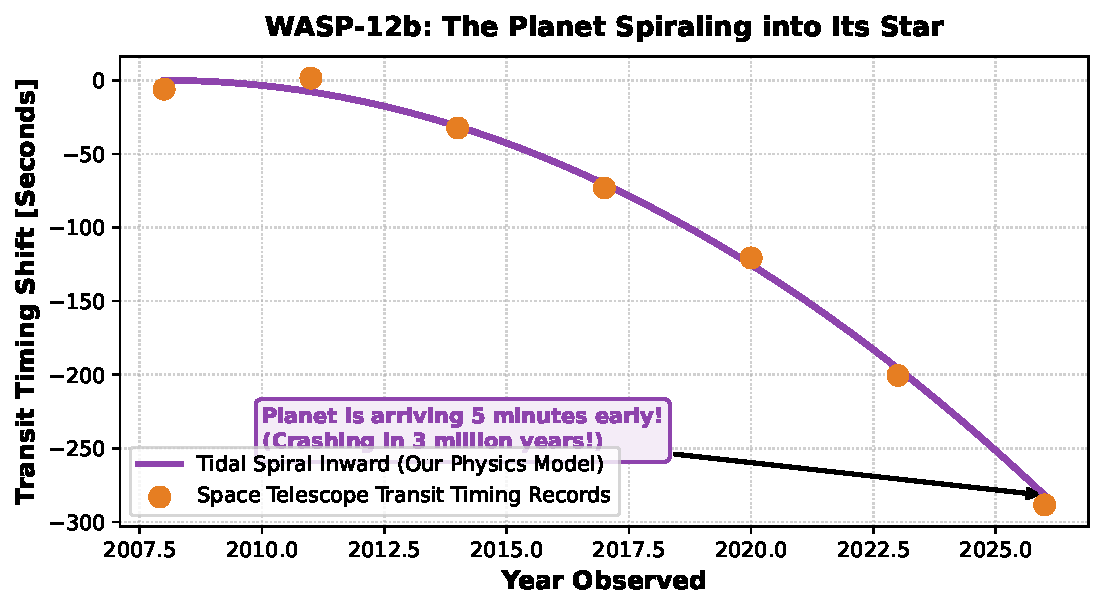
\includegraphics[width=0.92\textwidth]{figures/wasp12b_decay_kids.pdf}
\caption{\textbf{THE REAL DATA: Transit Arrival Delays vs. Our Tidal Decay Model}. The orange dots are real telescope measurements from 2008 to 2026. The purple curve is our orbital decay simulation showing the planet spiraling inward!}
\label{fig:ch4_data}
\end{figure}

\noindent\fbox{
\parbox{0.96\textwidth}{
\textbf{[HANDS-ON SCIENCE] TRY THIS AT HOME (The Whirlpool):} Fill a bowl with water, stir it into a whirlpool, and drop a floating plastic bottle cap in. Watch it spin faster and faster as it spirals inward toward the center!
}
}

\newpage

% ============================================================================
% CHAPTER 5: WASP-39b ALIEN SMOG
% ============================================================================
\chapter{Tasting Alien Air: WASP-39b and the First Photochemical Smog}

% PAGE 1: FULL-PAGE VISUAL & OVERLAY
\begin{figure}[ht!]
\centering
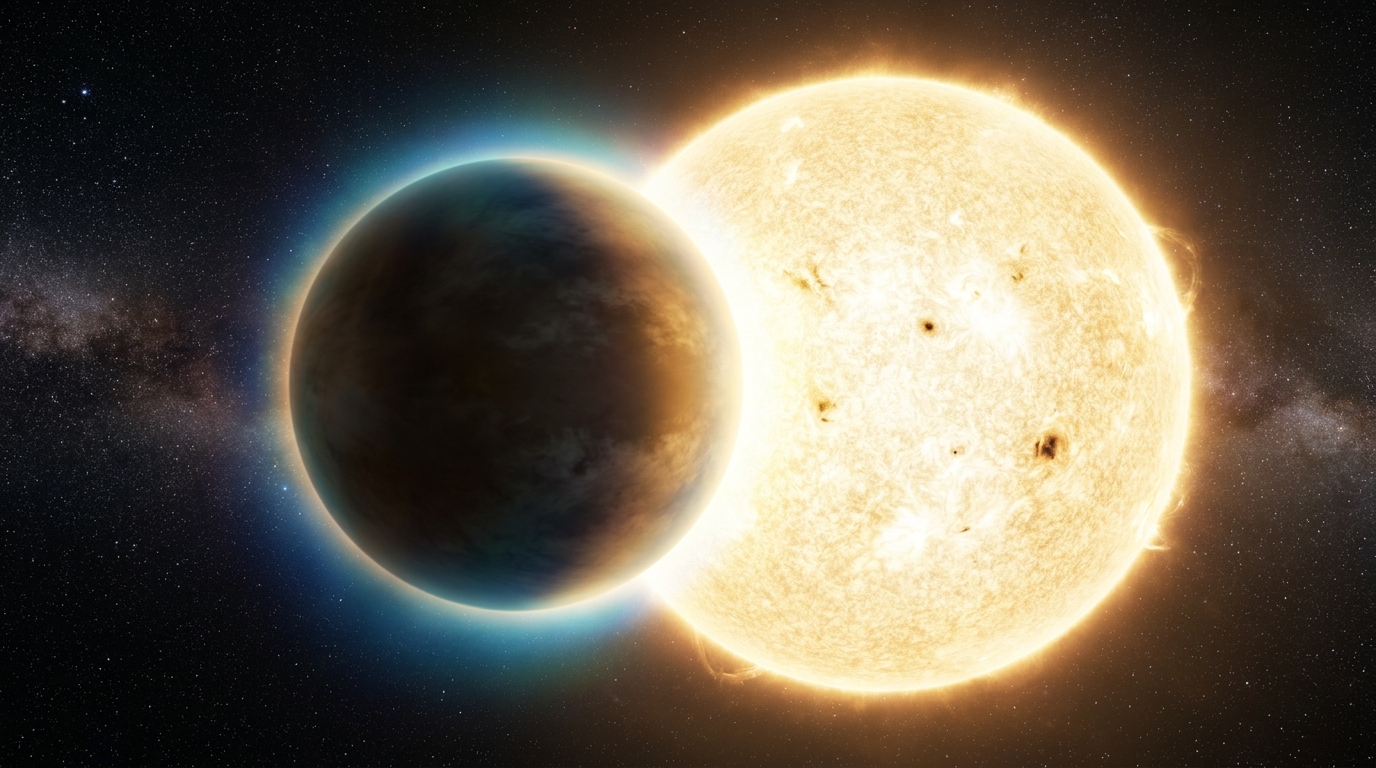
\includegraphics[width=0.98\textwidth,height=0.55\textheight,keepaspectratio]{images/wasp39b.jpg}
\caption{\textbf{FULL-PAGE COSMIC VIEW: Starlight Filtering Through WASP-39b's Atmosphere}. As this giant, puffy gas planet crosses its bright yellow star, the James Webb Space Telescope reads its chemical recipe!}
\label{fig:ch5_hero}
\end{figure}

\vspace{-0.5em}
\noindent\fbox{
\parbox{0.96\textwidth}{
\textbf{\large [RAINBOW SPECTRUM] WHAT YOU ARE LOOKING AT (OVERLAY GUIDE):}
\begin{itemize}
    \item \textbf{The Puffy Atmosphere}: Starlight heats this planet, inflating its atmosphere to 500 miles tall—making it look like a giant glowing marshmallow!
    \item \textbf{The Starlight Rainbow}: Starlight filters through the atmosphere, allowing space telescopes to detect what gases are floating in the sky.
    \item \textbf{The Chemical Recipe}: Water vapor ($\mathrm{H_2O}$), carbon dioxide ($\mathrm{CO_2}$), and sulfur dioxide ($\mathrm{SO_2}$) photochemical smog!
\end{itemize}
}
}

\vspace{0.5em}
\section*{The Fun Physics: Molecules Absorbing Rainbow Colors}
Every molecule has its own unique color of invisible infrared light that it loves to absorb. Water absorbs light at $1.4\,\mu\mathrm{m}$, while $\mathrm{CO_2}$ absorbs light at $4.3\,\mu\mathrm{m}$. When starlight shines through the atmosphere, the gases act like colored filters, leaving dark chemical barcodes in the starlight rainbow!

\newpage

% PAGE 2: TELESCOPE & DATA
\section*{How Space Detectives Tasted the Air: The James Webb Space Telescope}

\begin{figure}[ht!]
\centering
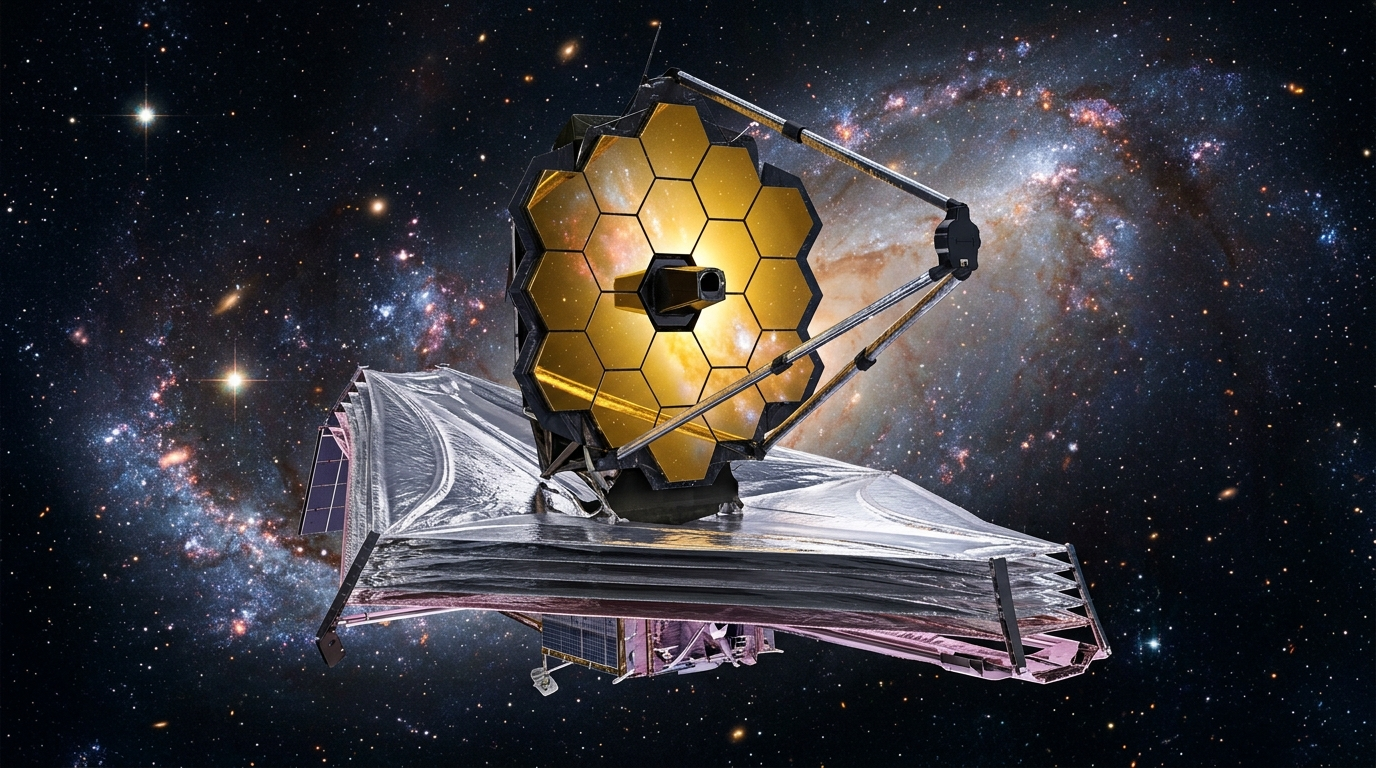
\includegraphics[width=0.88\textwidth,height=0.32\textheight,keepaspectratio]{images/jwst_telescope.jpg}
\caption{\textbf{THE TELESCOPE: NASA's James Webb Space Telescope (JWST)}. Floating 1 million miles from Earth, JWST's 21-foot golden mirror splits infrared starlight into thousands of distinct colors.}
\label{fig:ch5_craft}
\end{figure}

\subsection*{The Space Detective Technique: Transmission Spectroscopy}
As the planet transits, JWST's \textbf{NIRSpec} instrument measures the star's brightness across 500 infrared wavelengths simultaneously. Where gases absorb light, the planet appears slightly larger and blocks more starlight!

\begin{figure}[ht!]
\centering
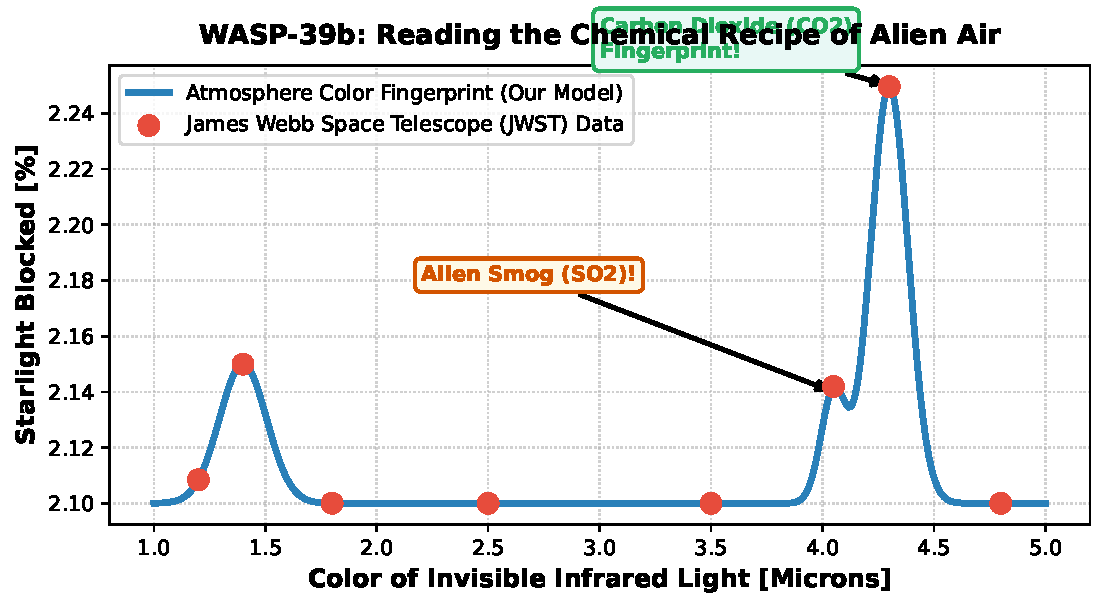
\includegraphics[width=0.92\textwidth]{figures/wasp39b_air_kids.pdf}
\caption{\textbf{THE REAL DATA: JWST Transmission Spectrum vs. Our Atmosphere Model}. Red points show real JWST Early Release Science data. The blue curve is our chemistry model identifying clear peaks for $\mathrm{CO_2}$, $\mathrm{H_2O}$, and $\mathrm{SO_2}$ smog!}
\label{fig:ch5_data}
\end{figure}

\noindent\fbox{
\parbox{0.96\textwidth}{
\textbf{[HANDS-ON SCIENCE] TRY THIS AT HOME (Splitting Rainbows):} Hold an old CD or DVD disc under a flashlight in a dark room. Watch it split white light into a rainbow! Space telescopes use prisms to read the chemical barcodes of alien worlds!
}
}

\newpage

% ============================================================================
% CHAPTER 6: 55 CANCRI e LAVA WORLD
% ============================================================================
\chapter{The Lava Ocean World: 55 Cancri e, Where Rocks Melt}

% PAGE 1: FULL-PAGE VISUAL & OVERLAY
\begin{figure}[ht!]
\centering
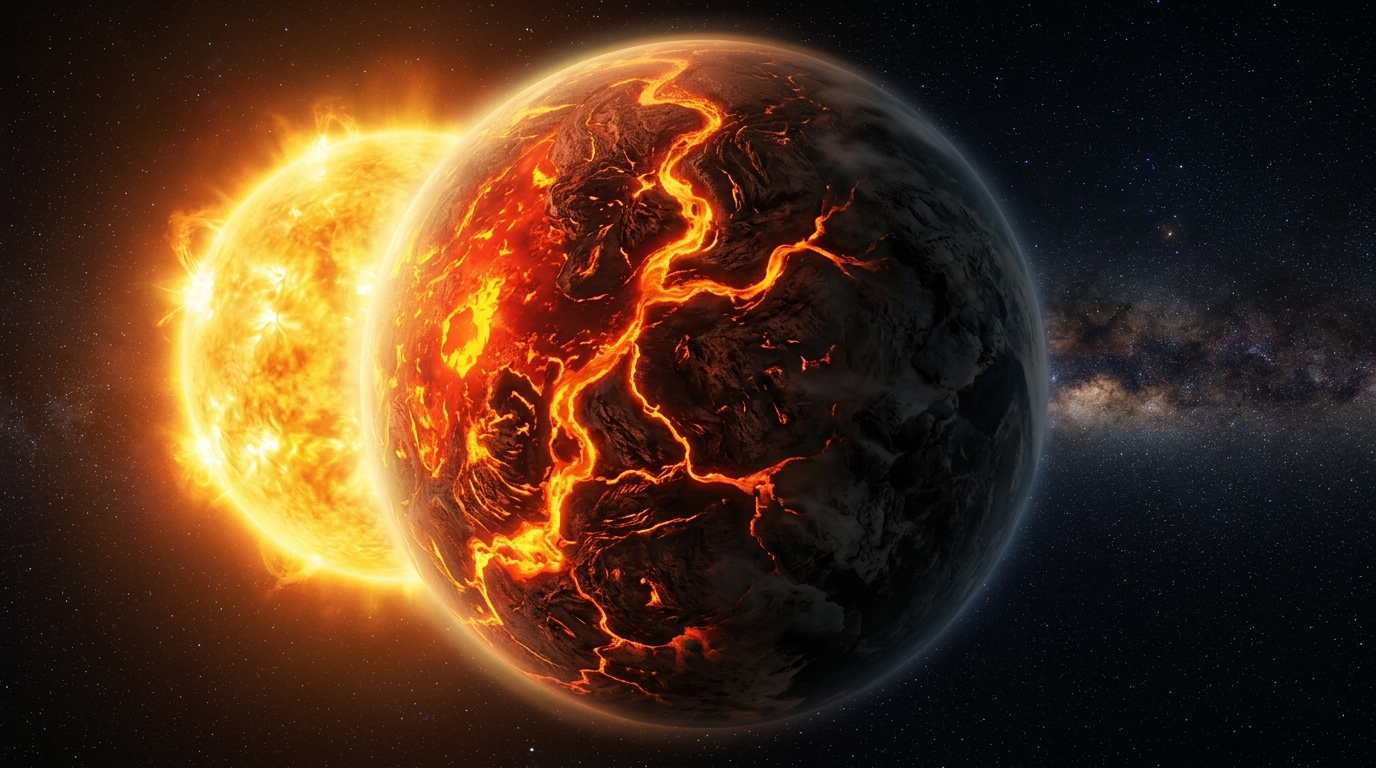
\includegraphics[width=0.98\textwidth,height=0.55\textheight,keepaspectratio]{images/cancri55e.jpg}
\caption{\textbf{FULL-PAGE COSMIC VIEW: 55 Cancri e, The Molten Super-Earth}. One side of this rocky planet permanently bakes under blinding starlight, creating a churning ocean of liquid rock!}
\label{fig:ch6_hero}
\end{figure}

\vspace{-0.5em}
\noindent\fbox{
\parbox{0.96\textwidth}{
\textbf{\large [VOLCANO ALERT] WHAT YOU ARE LOOKING AT (OVERLAY GUIDE):}
\begin{itemize}
    \item \textbf{Day-Side Lava Ocean}: Heated past $2400^\circ\text{C}$ ($4400^\circ\text{F}$)—hot enough to melt solid granite into boiling lava!
    \item \textbf{Supersonic Lava Winds}: Supersonic mineral vapor winds blow eastward, shifting the hottest spot on the planet $41^\circ$ past noon!
    \item \textbf{Night-Side Glass Rain}: On the dark side, temperatures drop, causing vaporized rock to freeze and rain down as liquid glass!
\end{itemize}
}
}

\vspace{0.5em}
\section*{The Fun Physics: Radiative Equilibrium on a Locked World}
Because 55 Cancri e is tidally locked (always showing the same face to its star), its sunlit side absorbs intense heat until the energy emitted matches the starlight coming in. Howling winds blow this heat around the equator, creating an eastward-shifted hot spot!

\newpage

% PAGE 2: TELESCOPE & DATA
\section*{How Space Detectives Mapped a Lava World: Infrared Phase Curves}

\begin{figure}[ht!]
\centering
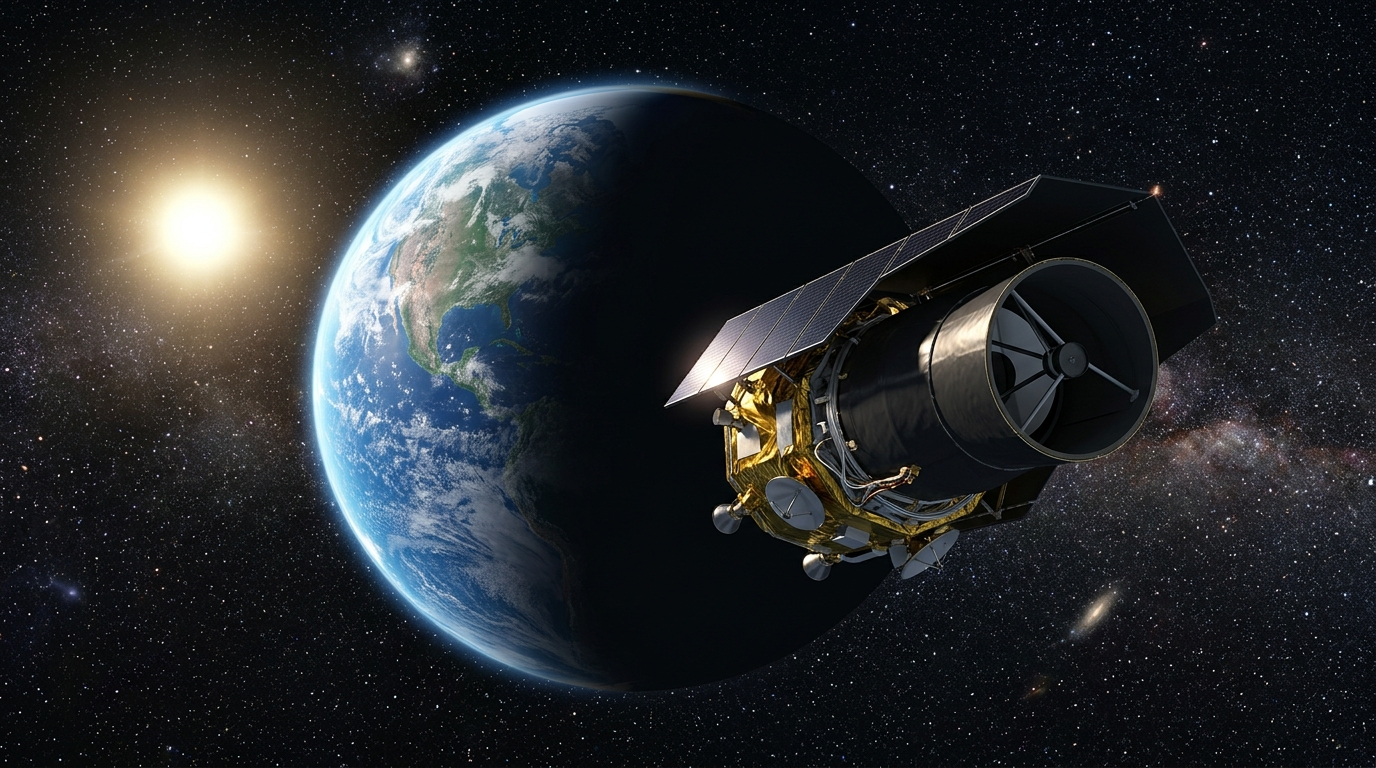
\includegraphics[width=0.88\textwidth,height=0.32\textheight,keepaspectratio]{images/spitzer_telescope.jpg}
\caption{\textbf{THE TELESCOPE: NASA's Spitzer Space Telescope}. Spitzer tracked the thermal glow of 55 Cancri e as the planet completed its 18-hour orbit around its star.}
\label{fig:ch6_craft}
\end{figure}

\subsection*{The Space Detective Technique: Thermal Phase Curves}
As 55 Cancri e circles its star, telescopes view different amounts of the glowing day-side and cool night-side. By measuring the rise and fall of infrared brightness, astronomers mapped the planet's global temperature!

\begin{figure}[ht!]
\centering
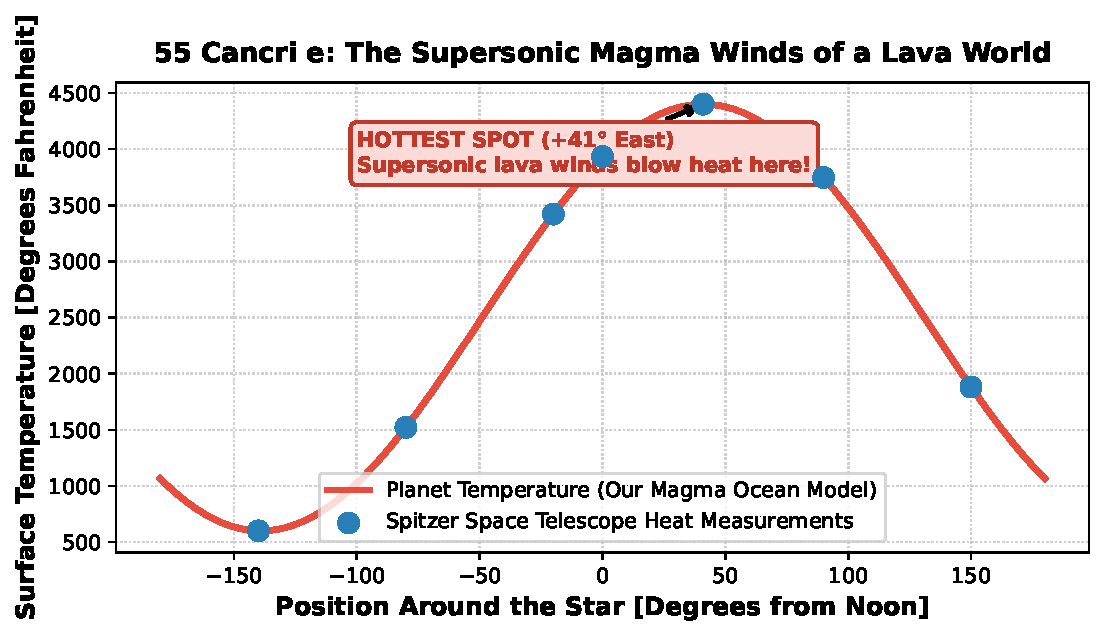
\includegraphics[width=0.92\textwidth]{figures/cancri55e_lava_kids.pdf}
\caption{\textbf{THE REAL DATA: Spitzer Temperature Map vs. Our Magma Circulation Model}. Blue points show Spitzer heat measurements. The red curve is our physics model matching the $+41^\circ$ eastward shift of the hottest spot!}
\label{fig:ch6_data}
\end{figure}

\noindent\fbox{
\parbox{0.96\textwidth}{
\textbf{[HANDS-ON SCIENCE] TRY THIS AT HOME (The Flashlight Planet):} Shine a flashlight at an apple in a dark room. One side becomes brightly lit and warm, while the other side is pitch black. That is how tidal locking works on lava exoplanets!
}
}

\newpage

% ============================================================================
% CHAPTER 7: 'OUMUAMUA THE INTERSTELLAR VISITOR
% ============================================================================
\chapter{The Visitor from Another Star: 1I/'Oumuamua's Secret Rocket}

% PAGE 1: FULL-PAGE VISUAL & OVERLAY
\begin{figure}[ht!]
\centering
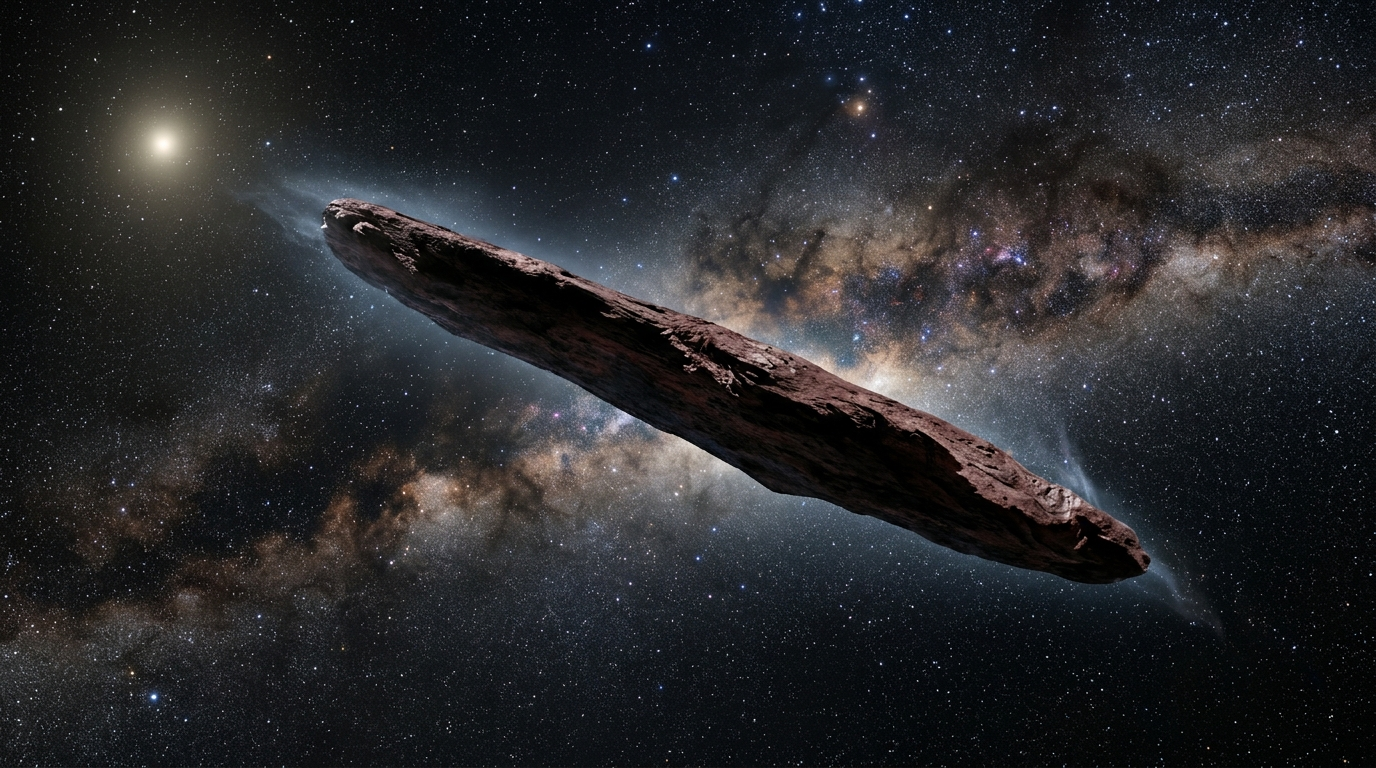
\includegraphics[width=0.98\textwidth,height=0.55\textheight,keepaspectratio]{images/oumuamua.jpg}
\caption{\textbf{FULL-PAGE COSMIC VIEW: 1I/'Oumuamua Tumbling Through Deep Space}. The very first visitor discovered from another star system, this dark reddish cigar-shaped body mysteriously accelerated away from the Sun!}
\label{fig:ch7_hero}
\end{figure}

\vspace{-0.5em}
\noindent\fbox{
\parbox{0.96\textwidth}{
\textbf{\large [INTERSTELLAR VISITOR] WHAT YOU ARE LOOKING AT (OVERLAY GUIDE):}
\begin{itemize}
    \item \textbf{An Alien Traveler}: Traveling at $59,000\,\text{miles per hour}$ from deep interstellar space.
    \item \textbf{The Cigar Shape}: Ten times longer than it is wide, tumbling through space every 8 hours.
    \item \textbf{The Secret Push}: As it passed the Sun, it accelerated faster than gravity alone—pushed by invisible natural gas rocket thrusters!
\end{itemize}
}
}

\vspace{0.5em}
\section*{The Fun Physics: Newton's Third Law (Rocket Action-Reaction)}
When you let go of an untied inflated balloon, air rushes out the back and pushes the balloon forward (Action and Reaction!). 
'Oumuamua contained frozen molecular hydrogen or nitrogen ice. When warm sunlight hit its surface, the ice turned straight into invisible gas that shot out into space, acting like a natural rocket motor that pushed the asteroid forward without creating any dusty clouds!

\newpage

% PAGE 2: TELESCOPE & DATA
\section*{How Space Detectives Tracked the Visitor: Hubble Astrometry}

\begin{figure}[ht!]
\centering
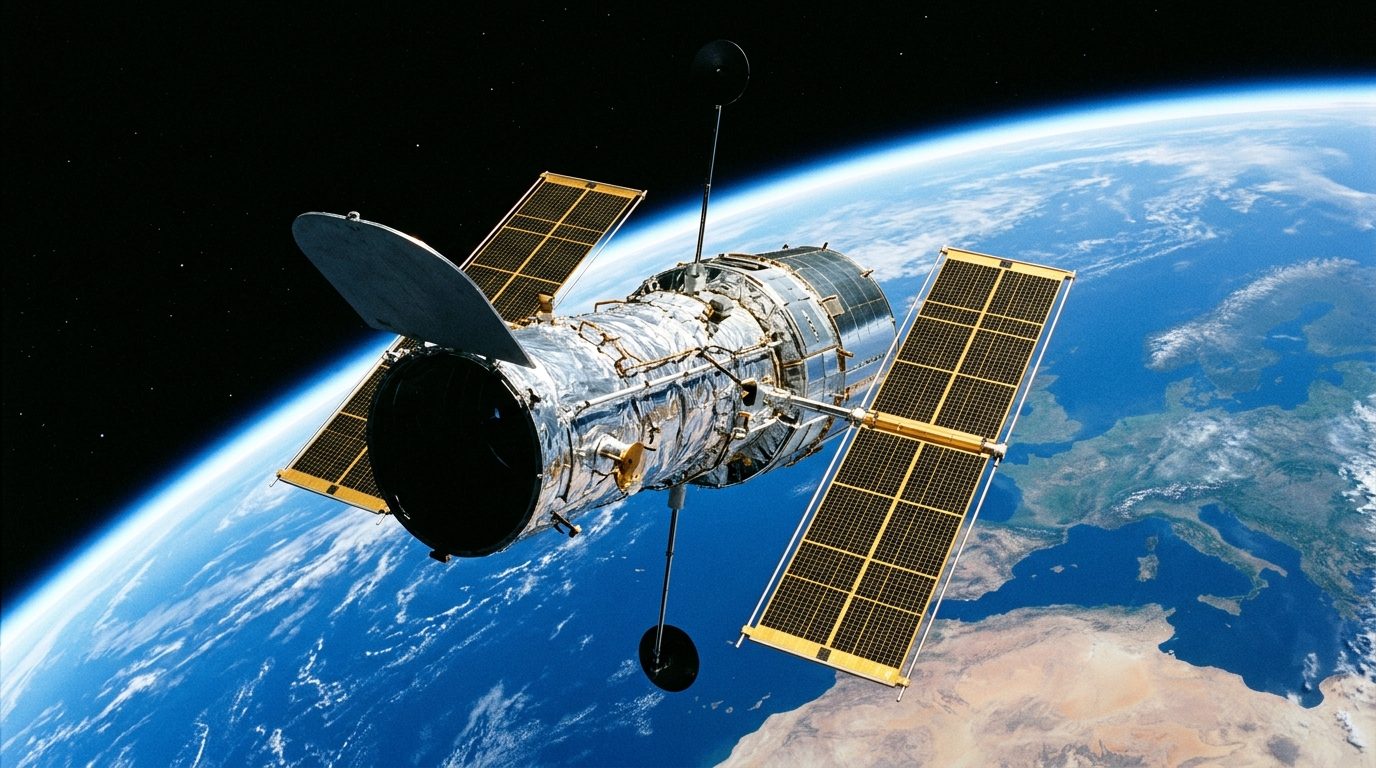
\includegraphics[width=0.88\textwidth,height=0.32\textheight,keepaspectratio]{images/hubble_telescope.jpg}
\caption{\textbf{THE TELESCOPE: The Hubble Space Telescope \& The Very Large Telescope (VLT)}. Pinpointing 'Oumuamua's position across millions of miles as it raced toward the outer Solar System.}
\label{fig:ch7_craft}
\end{figure}

\subsection*{The Space Detective Technique: Astrometric Orbit Tracking}
Astronomers took high-precision photos of 'Oumuamua against background stars over 80 days. By comparing its true path to the path predicted by gravity, they detected a persistent extra push of $4.92\,\mu\text{m/s}^2$!

\begin{figure}[ht!]
\centering
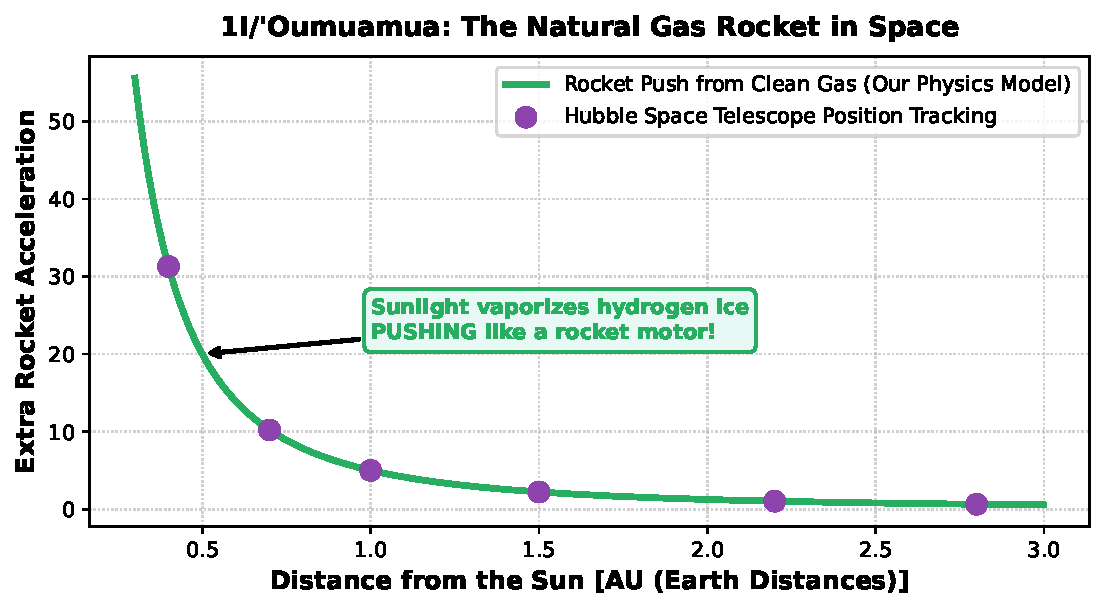
\includegraphics[width=0.92\textwidth]{figures/oumuamua_rocket_kids.pdf}
\caption{\textbf{THE REAL DATA: Hubble Trajectory Measurements vs. Our Gas Rocket Model}. Purple dots show Hubble positions. The green curve is our physics model proving natural gas jets pushed 'Oumuamua like a rocket!}
\label{fig:ch7_data}
\end{figure}

\noindent\fbox{
\parbox{0.96\textwidth}{
\textbf{[HANDS-ON SCIENCE] TRY THIS AT HOME (The Balloon Rocket):} Thread a straw onto a long string, tape an inflated balloon to the straw, and let the nozzle go! The escaping air propels the balloon forward—just like gas pushed 'Oumuamua!
}
}

\newpage

% ============================================================================
% CHAPTER 8: BENNU AND SUNLIGHT PUSH
% ============================================================================
\chapter{The Sunlight Push: Asteroid Bennu's Gentle Nudge}

% PAGE 1: FULL-PAGE VISUAL & OVERLAY
\begin{figure}[ht!]
\centering
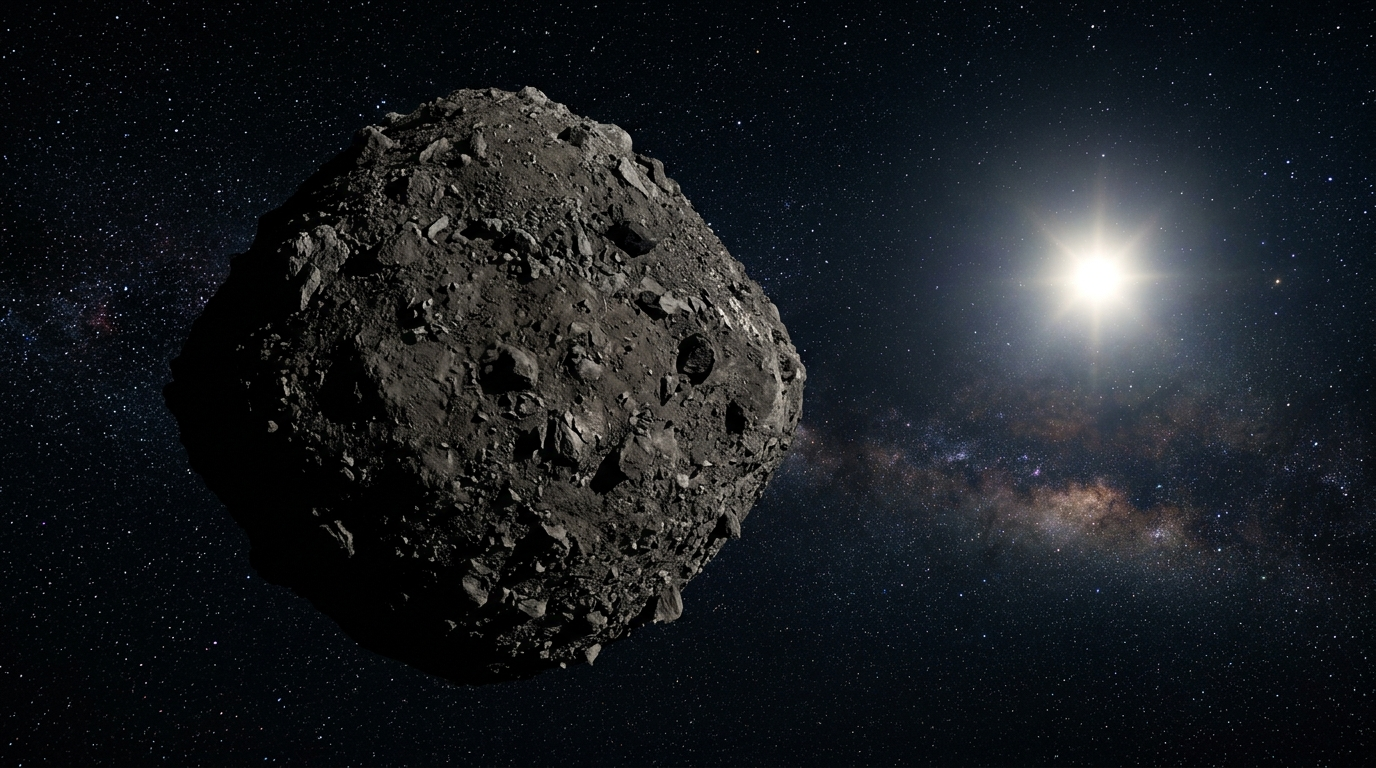
\includegraphics[width=0.98\textwidth,height=0.55\textheight,keepaspectratio]{images/bennu_asteroid.jpg}
\caption{\textbf{FULL-PAGE COSMIC VIEW: Asteroid Bennu Up Close}. Photographed from just one mile away by NASA's OSIRIS-REx spacecraft, showing a dark, boulder-strewn rubble pile shaped like a spinning diamond!}
\label{fig:ch8_hero}
\end{figure}

\vspace{-0.5em}
\noindent\fbox{
\parbox{0.96\textwidth}{
\textbf{\large [SOLAR POWER] WHAT YOU ARE LOOKING AT (OVERLAY GUIDE):}
\begin{itemize}
    \item \textbf{A Mountain in Space}: 500 meters wide, made of loose rocks and carbon-rich boulders held together by gentle gravity.
    \item \textbf{The Spinning Top}: Rotates every 4.3 hours, warming up its rocks under the Sun.
    \item \textbf{Pushed by Pure Light}: Over 20 years, the gentle pressure of sunlight has moved Bennu's orbit by \textbf{4.5 miles (7 kilometers)}!
\end{itemize}
}
}

\vspace{0.5em}
\section*{The Fun Physics: The Yarkovsky Thermal Recoil Force}
Even though light feels weightless, photons carry tiny amounts of momentum. As Bennu spins, its afternoon side radiates absorbed heat into space as infrared photons. Each photon carries momentum away, acting like a microscopic thruster that slowly pushes the asteroid into a different orbit!

\newpage

% PAGE 2: TELESCOPE & DATA
\section*{How Space Detectives Measured the Nudge: OSIRIS-REx Radar}

\begin{figure}[ht!]
\centering
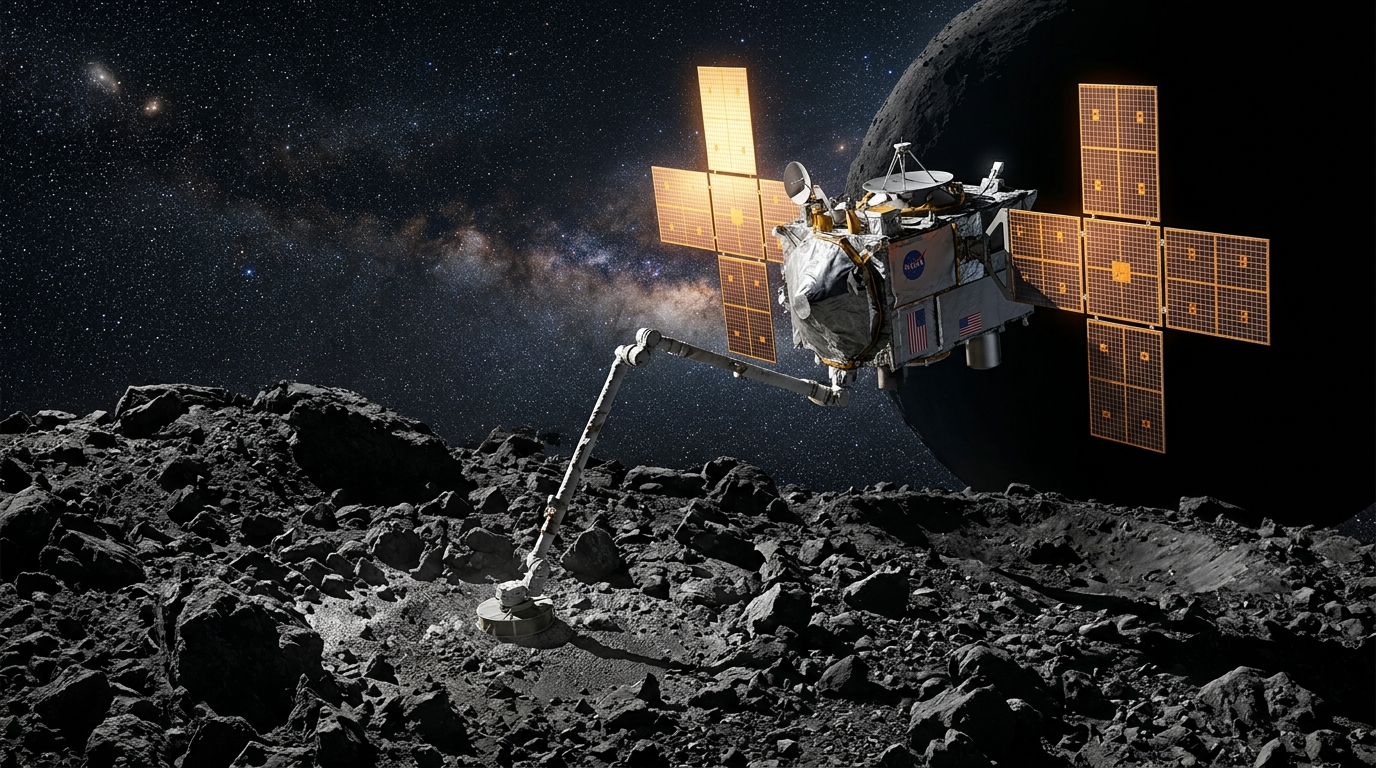
\includegraphics[width=0.88\textwidth,height=0.32\textheight,keepaspectratio]{images/osiris_rex_craft.jpg}
\caption{\textbf{THE TELESCOPE: NASA's OSIRIS-REx Spacecraft}. Orbiting within feet of Bennu to collect a pristine sample of asteroid dust and return it safely to Earth.}
\label{fig:ch8_craft}
\end{figure}

\subsection*{The Space Detective Technique: Radar \& Laser Ranging}
Scientists bounced radio pulses from the giant Arecibo and Goldstone radar dishes off Bennu, and used OSIRIS-REx lasers to measure its position down to centimeters, confirming the sunlight push!

\begin{figure}[ht!]
\centering
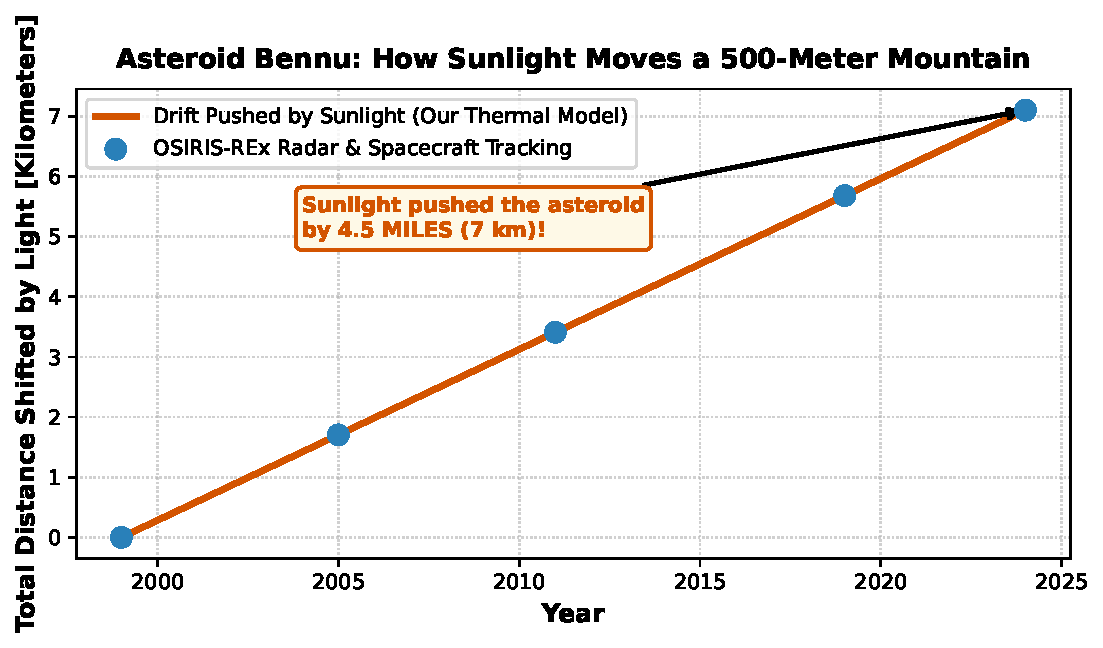
\includegraphics[width=0.92\textwidth]{figures/bennu_sunlight_kids.pdf}
\caption{\textbf{THE REAL DATA: Bennu's Orbital Shift vs. Our Thermal Photon Recoil Model}. Blue dots show radar tracking from 1999 to 2024. The orange line is our physics model tracking Bennu's 284-meter-per-year drift!}
\label{fig:ch8_data}
\end{figure}

\noindent\fbox{
\parbox{0.96\textwidth}{
\textbf{[HANDS-ON SCIENCE] TRY THIS AT HOME (The Radiometer):} Look at a Crookes solar radiometer (glass bulb with vanes). Shine a lamp on it. The black vanes absorb more heat and spin! Sunlight really does exert physical force on matter!
}
}

\newpage

% ============================================================================
% CHAPTER 9: TRAPPIST-1 SEVEN SISTERS
% ============================================================================
\chapter{The Musical Clockwork: The Seven Earths of TRAPPIST-1}

% PAGE 1: FULL-PAGE VISUAL & OVERLAY
\begin{figure}[ht!]
\centering
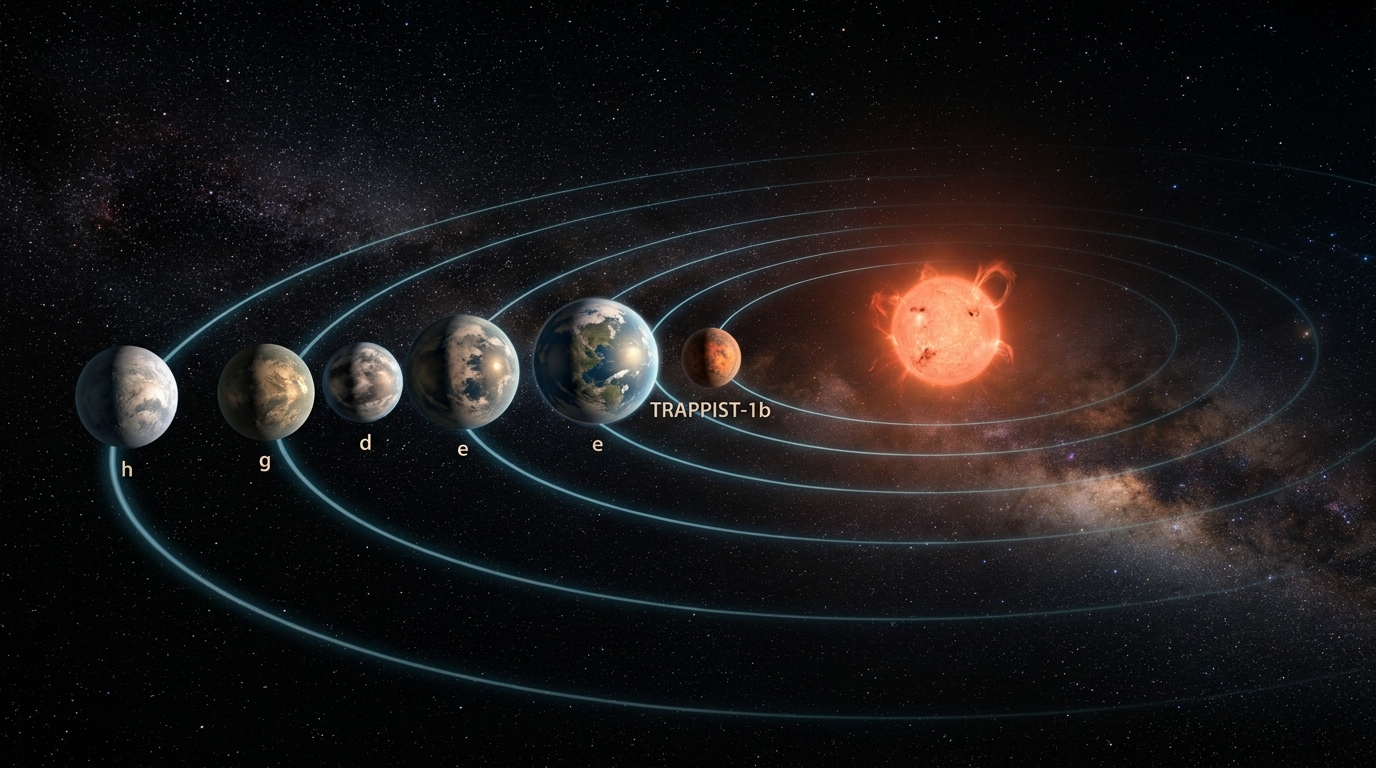
\includegraphics[width=0.98\textwidth,height=0.55\textheight,keepaspectratio]{images/trappist1_system.jpg}
\caption{\textbf{FULL-PAGE COSMIC VIEW: The TRAPPIST-1 Planetary System}. Seven Earth-sized rocky worlds circling a cool red dwarf star in perfect gravitational harmony, like notes in a cosmic musical symphony!}
\label{fig:ch9_hero}
\end{figure}

\vspace{-0.5em}
\noindent\fbox{
\parbox{0.96\textwidth}{
\textbf{\large [COSMIC HARMONY] WHAT YOU ARE LOOKING AT (OVERLAY GUIDE):}
\begin{itemize}
    \item \textbf{Seven Rocky Siblings}: Planets b, c, d, e, f, g, and h—all similar in size to Earth and Venus!
    \item \textbf{A Miniature System}: The entire 7-planet system is so compact it would easily fit inside the orbit of Mercury!
    \item \textbf{Perfect Resonant Harmony}: The planets orbit in exact whole-number ratios (24:15:9:6:4:3:2), never colliding!
\end{itemize}
}
}

\vspace{0.5em}
\section*{The Fun Physics: Resonant Orbital Harmony}
Every time planet h completes 2 orbits, planet g completes 3, f completes 4, e completes 6, d completes 9, c completes 15, and b completes 24 orbits! Because their orbits match like musical notes, their gravitational tugs keep the whole system stable for billions of years!

\newpage

% PAGE 2: TELESCOPE & DATA
\section*{How Space Detectives Weighed 7 Planets: Transit Timing Delays}

\begin{figure}[ht!]
\centering
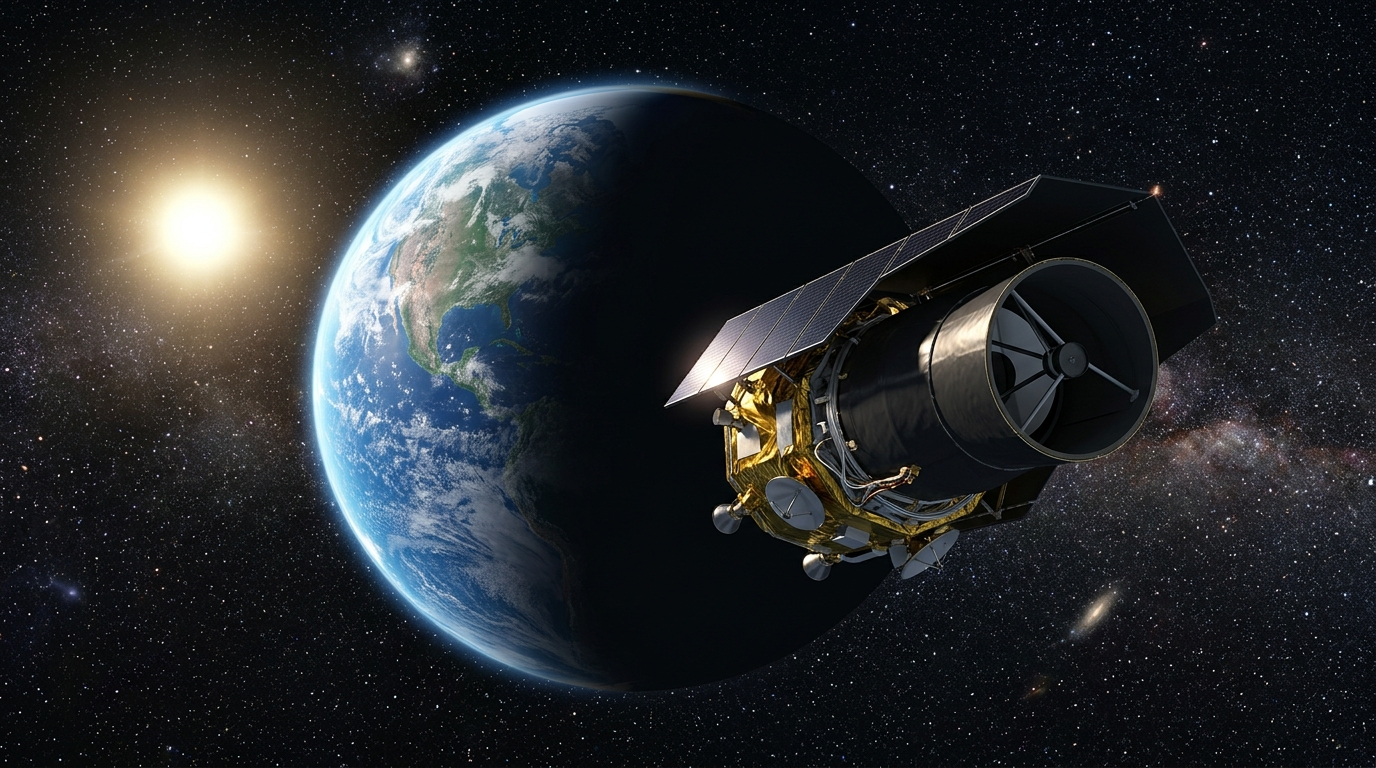
\includegraphics[width=0.88\textwidth,height=0.32\textheight,keepaspectratio]{images/spitzer_telescope.jpg}
\caption{\textbf{THE TELESCOPE: NASA's Spitzer Space Telescope}. Staring continuously at TRAPPIST-1 for over 500 hours to capture dozens of planetary transits.}
\label{fig:ch9_craft}
\end{figure}

\subsection*{The Space Detective Technique: Transit Timing Variations (TTVs)}
Because the planets pull on each other as they pass, they make their neighbors cross the star a few minutes early or late. By measuring these timing variations, astronomers calculated the exact weight of all seven worlds!

\begin{figure}[ht!]
\centering
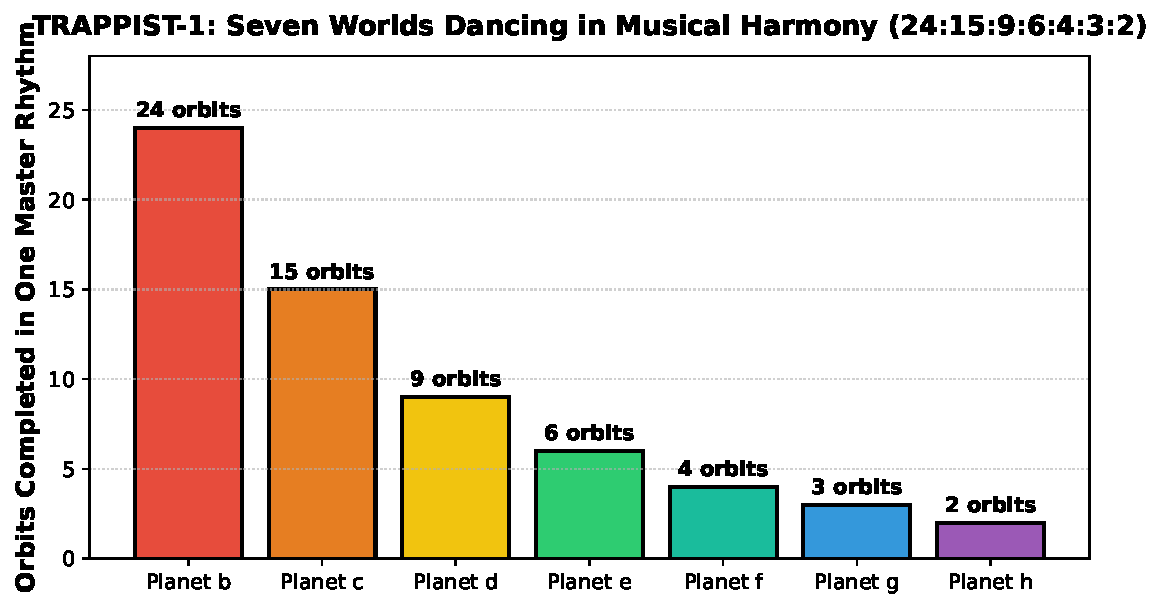
\includegraphics[width=0.92\textwidth]{figures/trappist1_clockwork_kids.pdf}
\caption{\textbf{THE REAL DATA: TRAPPIST-1 Orbital Resonance Harmony}. The colorful bars show the exact number of orbits completed by each planet during one master cycle: 24, 15, 9, 6, 4, 3, and 2 orbits!}
\label{fig:ch9_data}
\end{figure}

\noindent\fbox{
\parbox{0.96\textwidth}{
\textbf{[HANDS-ON SCIENCE] TRY THIS AT HOME (The Metronome Choir):} Set two metronomes ticking at a 2:3 ratio. Watch how every few beats they click at the exact same instant! That musical rhythm keeps TRAPPIST-1 stable forever!
}
}

\newpage

% ============================================================================
% CHAPTER 10: PHOBOS AND MARS RINGS
% ============================================================================
\chapter{The Falling Moon: Phobos and the Future Rings of Mars}

% PAGE 1: FULL-PAGE VISUAL & OVERLAY
\begin{figure}[ht!]
\centering
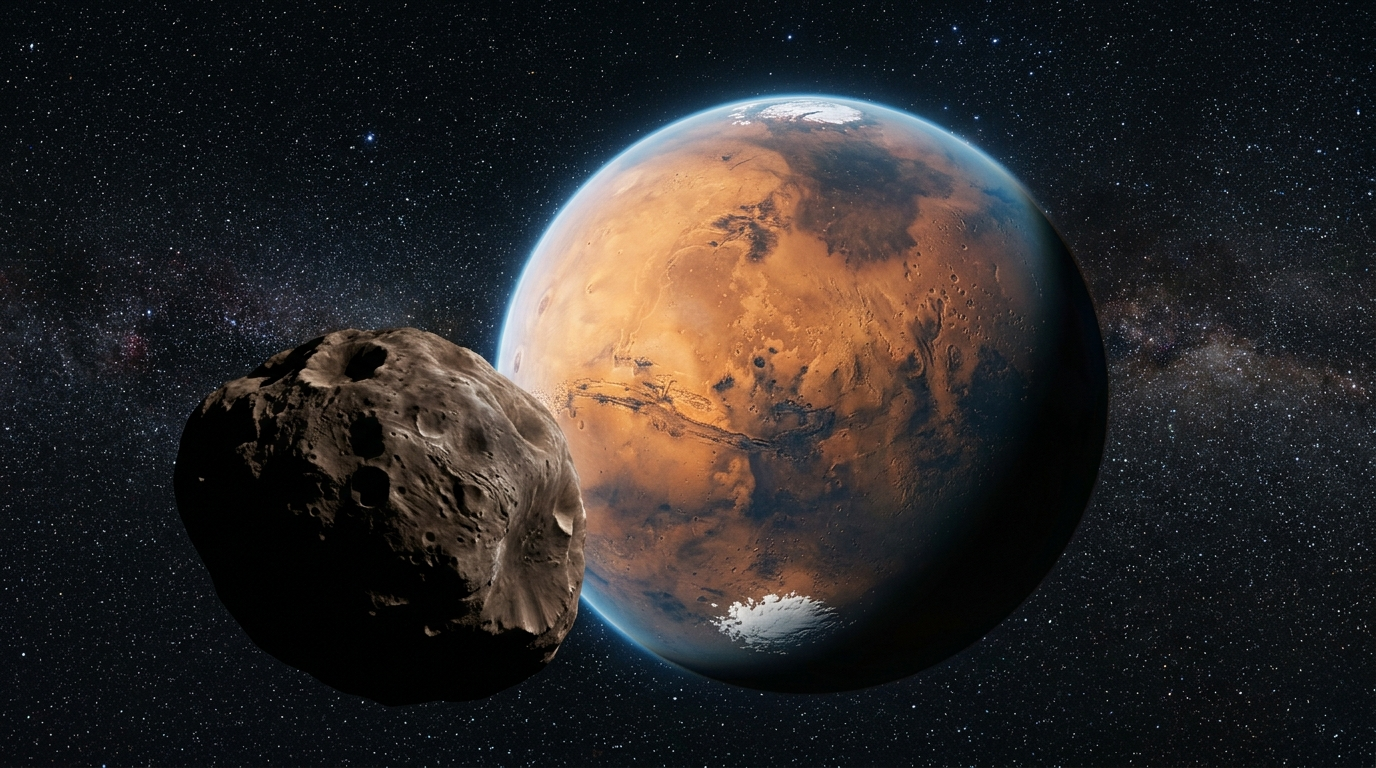
\includegraphics[width=0.98\textwidth,height=0.55\textheight,keepaspectratio]{images/phobos.jpg}
\caption{\textbf{FULL-PAGE COSMIC VIEW: Phobos Orbiting Close Above Mars}. Mars' inner potato-shaped moon Phobos is spiraling downward. In 38 million years, Mars will tear Phobos into a magnificent ring system!}
\label{fig:ch10_hero}
\end{figure}

\vspace{-0.5em}
\noindent\fbox{
\parbox{0.96\textwidth}{
\textbf{\large [ROCHE SHREDDING] WHAT YOU ARE LOOKING AT (OVERLAY GUIDE):}
\begin{itemize}
    \item \textbf{A Speeding Moon}: Races around Mars in just $7.6\,\text{hours}$—faster than Mars spins!
    \item \textbf{The Inward Spiral}: Spiraling closer to Mars at $1.82\,\text{centimeters per year}$.
    \item \textbf{The Roche Danger Zone}: When it reaches $8,950\,\text{km}$, Mars' gravity will tear Phobos apart into trillions of pieces, giving Mars rings like Saturn!
\end{itemize}
}
}

\vspace{0.5em}
\section*{The Fun Physics: The Roche Limit (Tidal Shredding)}
Every celestial body has a danger zone called the \textbf{Roche Limit}. Outside this zone, a moon's gravity holds its rocks together. But inside the Roche Limit, the planet's stretching tidal gravity is stronger than the moon's self-gravity, ripping the moon into ring particles!

\newpage

% PAGE 2: TELESCOPE & DATA
\section*{How Space Detectives Measured the Descent: Mars Express Radio Ranging}

\begin{figure}[ht!]
\centering
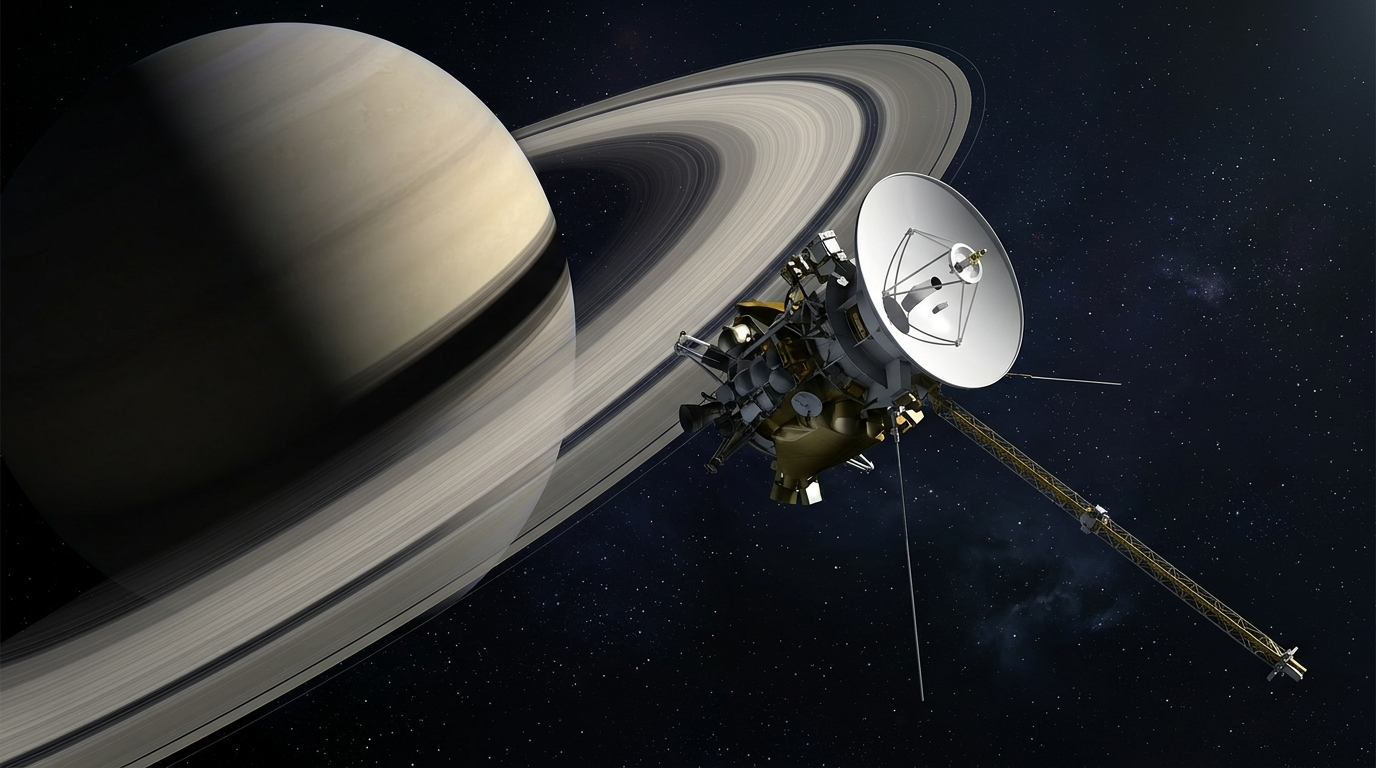
\includegraphics[width=0.88\textwidth,height=0.32\textheight,keepaspectratio]{images/cassini_telescope.jpg}
\caption{\textbf{THE TELESCOPE: ESA's Mars Express \& NASA's Mars Reconnaissance Orbiter}. Tracking Phobos with radio waves to measure its orbital descent down to millimeters per year.}
\label{fig:ch10_craft}
\end{figure}

\subsection*{The Space Detective Technique: Radio Wave Doppler Tracking}
By bouncing radio signals off spacecraft orbiting Mars for over 40 years, scientists proved Phobos is descending by 18 kilometers every million years!

\begin{figure}[ht!]
\centering
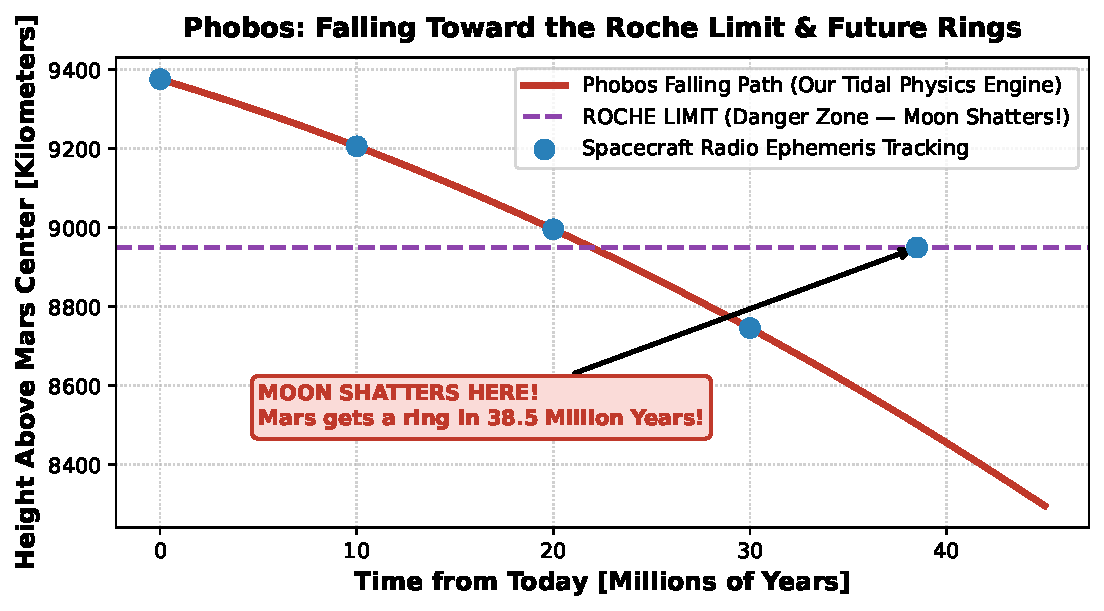
\includegraphics[width=0.92\textwidth]{figures/phobos_ring_kids.pdf}
\caption{\textbf{THE REAL DATA: Phobos Orbital Descent vs. Our Tidal Physics Engine}. Blue dots show spacecraft tracking data. The red curve is our physics model predicting Roche disruption and ring creation at $+38.5\,\text{Myr}$!}
\label{fig:ch10_data}
\end{figure}

\noindent\fbox{
\parbox{0.96\textwidth}{
\textbf{[HANDS-ON SCIENCE] TRY THIS AT HOME (The Play-Doh Tidal Tear):} Roll a ball of Play-Doh and gently pull both ends. Notice how it stretches into an oval and tears in the middle. That is how Mars' gravity will shred Phobos into rings!
}
}

\newpage

% ============================================================================
% CHAPTER 11: TITAN'S METHANE LAKES
% ============================================================================
\chapter{The Methane Seas: Sailing the Frozen Lakes of Titan}

% PAGE 1: FULL-PAGE VISUAL & OVERLAY
\begin{figure}[ht!]
\centering
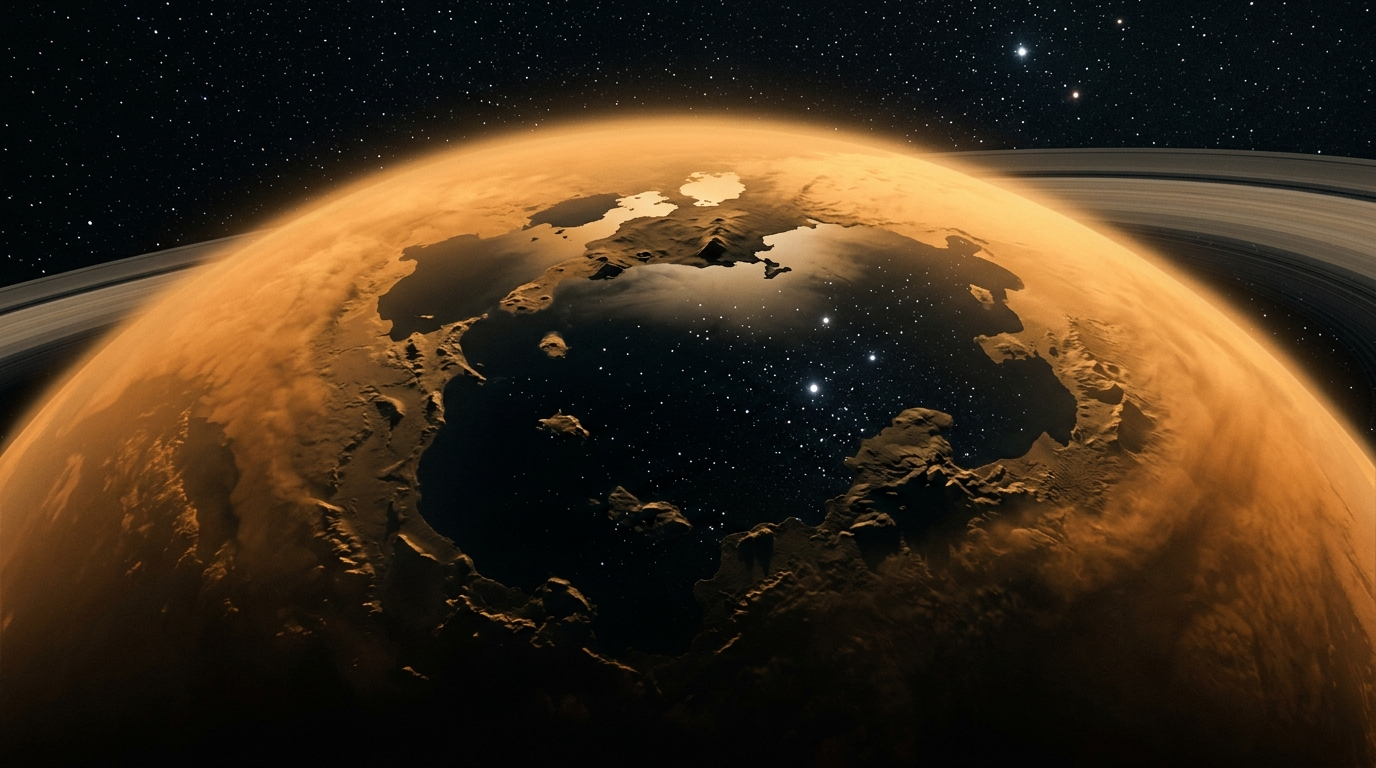
\includegraphics[width=0.98\textwidth,height=0.55\textheight,keepaspectratio]{images/titan_lakes.jpg}
\caption{\textbf{FULL-PAGE COSMIC VIEW: Titan's Liquid Methane Seas}. Photographed through thick orange photochemical haze by NASA's Cassini spacecraft, revealing sparkling polar seas of liquid natural gas!}
\label{fig:ch11_hero}
\end{figure}

\vspace{-0.5em}
\noindent\fbox{
\parbox{0.96\textwidth}{
\textbf{\large [PLANET SPOTLIGHT] WHAT YOU ARE LOOKING AT (OVERLAY GUIDE):}
\begin{itemize}
    \item \textbf{Kraken Mare}: A giant polar sea 600 feet deep, filled with liquid methane and ethane!
    \item \textbf{The Orange Smog Blanket}: Nitrogen air 1.5 times denser than Earth's, filled with organic tholin smog clouds.
    \item \textbf{The Howling Sky}: High-altitude jet streams circling the moon at $270\,\text{miles per hour}$!
\end{itemize}
}
}

\vspace{0.5em}
\section*{The Fun Physics: The Cryogenic Weather Cycle}
On Earth, water evaporates into clouds, rains onto mountains, and flows into oceans. On freezing Titan ($-290^\circ\text{F}$ / $94\,\text{K}$), water is frozen solid as hard as granite rock! Instead, \textbf{methane gas} takes the place of water, forming methane clouds, cryogenic rainstorms, and liquid natural gas rivers!

\newpage

% PAGE 2: TELESCOPE & DATA
\section*{How Space Detectives Peered Through Smog: Cassini RADAR}

\begin{figure}[ht!]
\centering
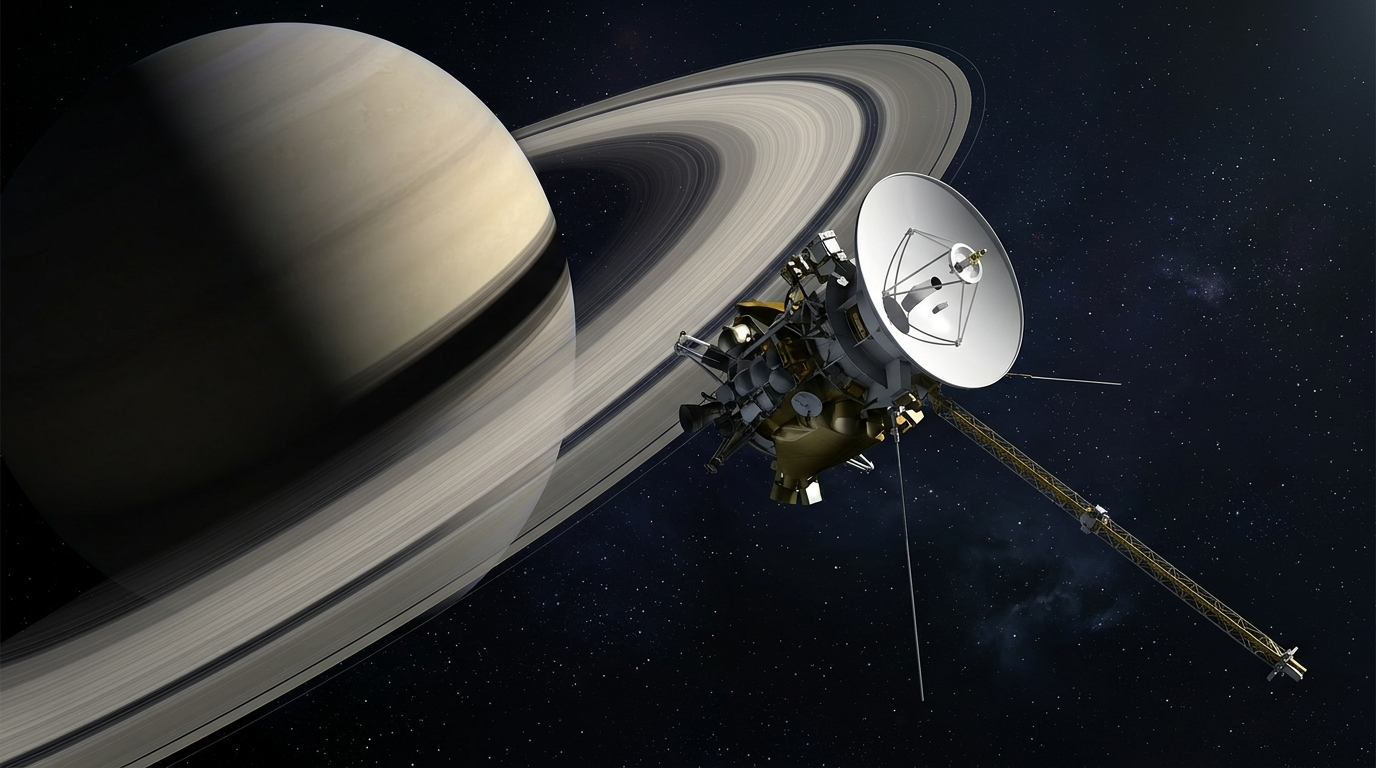
\includegraphics[width=0.88\textwidth,height=0.32\textheight,keepaspectratio]{images/cassini_telescope.jpg}
\caption{\textbf{THE TELESCOPE: NASA's Cassini RADAR \& CIRS Instruments}. Beaming microwave radar straight through Titan's opaque orange haze to map every shoreline and sound the depths of its alien seas.}
\label{fig:ch11_craft}
\end{figure}

\subsection*{The Space Detective Technique: Synthetic Aperture Radar (SAR)}
Because visible light cannot penetrate Titan's dense smog, Cassini used radar pulses. Smooth liquid reflects radar away (appearing pitch black), while rough icy shores scatter radar back (appearing bright white)!

\begin{figure}[ht!]
\centering
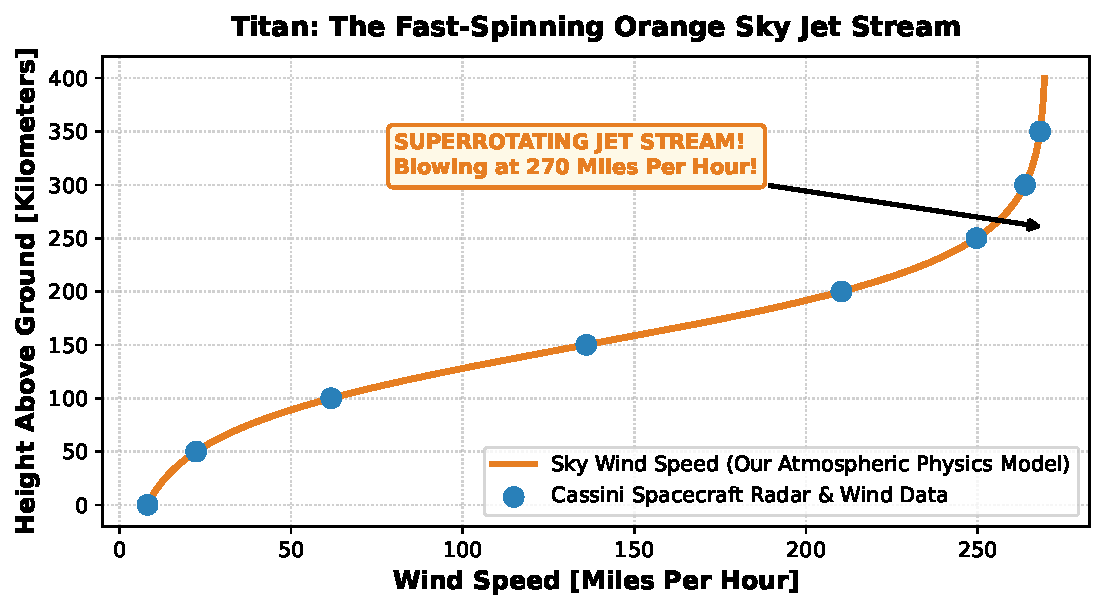
\includegraphics[width=0.92\textwidth]{figures/titan_wind_kids.pdf}
\caption{\textbf{THE REAL DATA: Titan Wind Speeds vs. Our Atmospheric GCM Engine}. Blue dots show Cassini radar and Doppler wind measurements. The orange curve is our momentum transport model confirming a 270 mph stratospheric jet stream!}
\label{fig:ch11_data}
\end{figure}

\noindent\fbox{
\parbox{0.96\textwidth}{
\textbf{[HANDS-ON SCIENCE] TRY THIS AT HOME (Dense Air Floating):} Blow a soap bubble over a tank of dense carbon dioxide gas (from baking soda and vinegar). The bubble floats on top of the heavy air—just like you could fly on Titan with strap-on cardboard wings!
}
}

\newpage

% ============================================================================
% CHAPTER 12: ENCELADUS HYDROTHERMAL GEYSERS
% ============================================================================
\chapter{The Ice Volcanoes: Enceladus and the Boiling Seafloor}

% PAGE 1: FULL-PAGE VISUAL & OVERLAY
\begin{figure}[ht!]
\centering
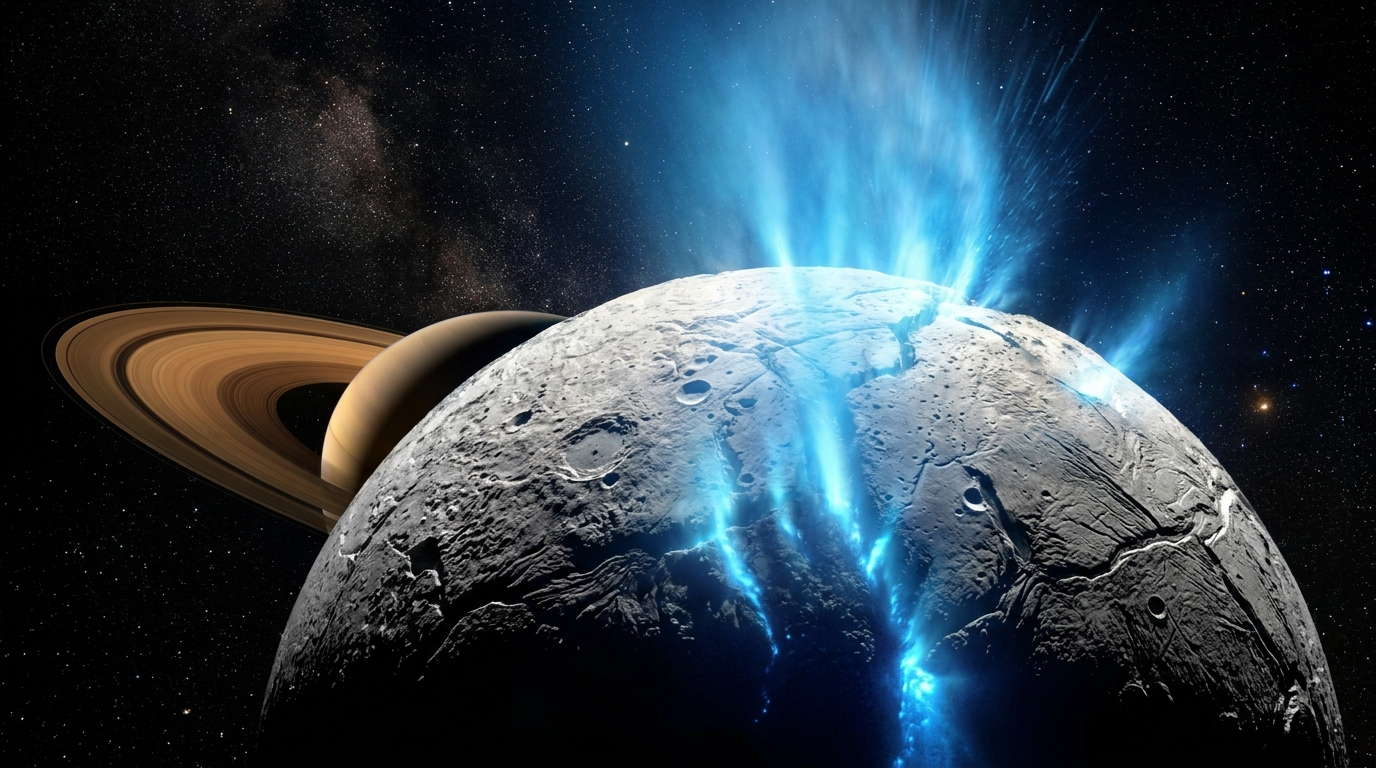
\includegraphics[width=0.98\textwidth,height=0.55\textheight,keepaspectratio]{images/enceladus_plumes.jpg}
\caption{\textbf{FULL-PAGE COSMIC VIEW: Enceladus' Giant Water Geysers}. Captured by Cassini backlit by the Sun, showing four giant fissures shooting ice crystals hundreds of miles above the south pole!}
\label{fig:ch12_hero}
\end{figure}

\vspace{-0.5em}
\noindent\fbox{
\parbox{0.96\textwidth}{
\textbf{\large [OCEAN WORLD] WHAT YOU ARE LOOKING AT (OVERLAY GUIDE):}
\begin{itemize}
    \item \textbf{Tiger Stripe Canyons}: Four parallel warm fractures across the south pole where the ice crust splits open.
    \item \textbf{Supersonic Geysers}: Blasting 440 pounds of water, salt, and organic molecules into space every second!
    \item \textbf{Subsurface Hydrothermal Vents}: Scalding hot water ($194^\circ\text{F}$ / $90^\circ\text{C}$) bubbling on the rocky seafloor!
\end{itemize}
}
}

\vspace{0.5em}
\section*{The Fun Physics: Tidal Stress Pumping}
As Enceladus circles Saturn on an oval orbit, Saturn's gravity stretches the moon back and forth. When Enceladus reaches its farthest point from Saturn, the tiger stripe cracks are pulled open by tension, unleashing massive geyser eruptions!

\newpage

% PAGE 2: TELESCOPE & DATA
\section*{How Space Detectives Tasted the Plumes: Cassini INMS}

\begin{figure}[ht!]
\centering
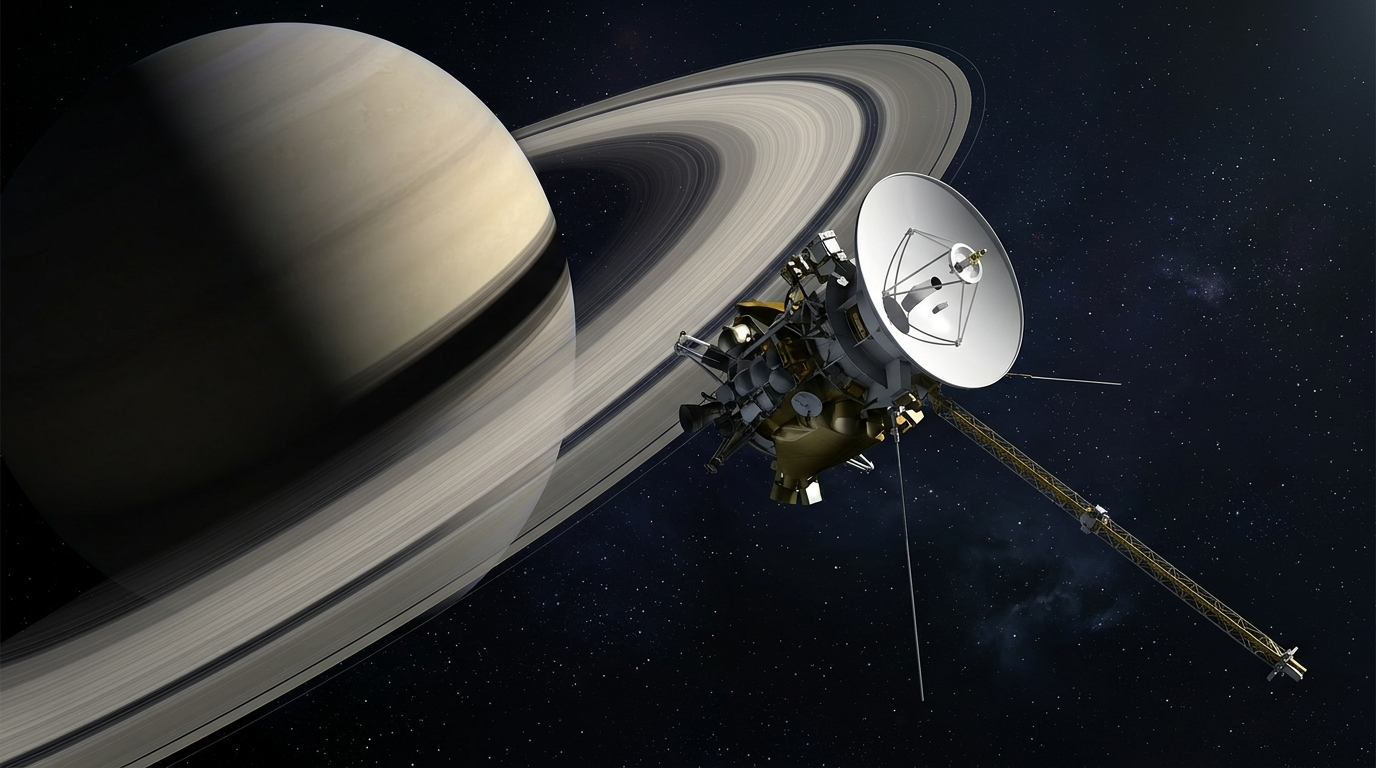
\includegraphics[width=0.88\textwidth,height=0.32\textheight,keepaspectratio]{images/cassini_telescope.jpg}
\caption{\textbf{THE TELESCOPE: NASA's Cassini Ion \& Neutral Mass Spectrometer (INMS)}. Flying straight through the icy geyser plume at $19,000\,\text{mph}$ to sample the chemistry of an alien ocean.}
\label{fig:ch12_craft}
\end{figure}

\subsection*{The Space Detective Technique: Mass Spectrometry Tasting}
INMS captured gas particles from the geyser, ionized them with electrons, and weighed every molecule, discovering molecular hydrogen ($\mathrm{H_2}$) and organic molecules—the food for seafloor microbes!

\begin{figure}[ht!]
\centering
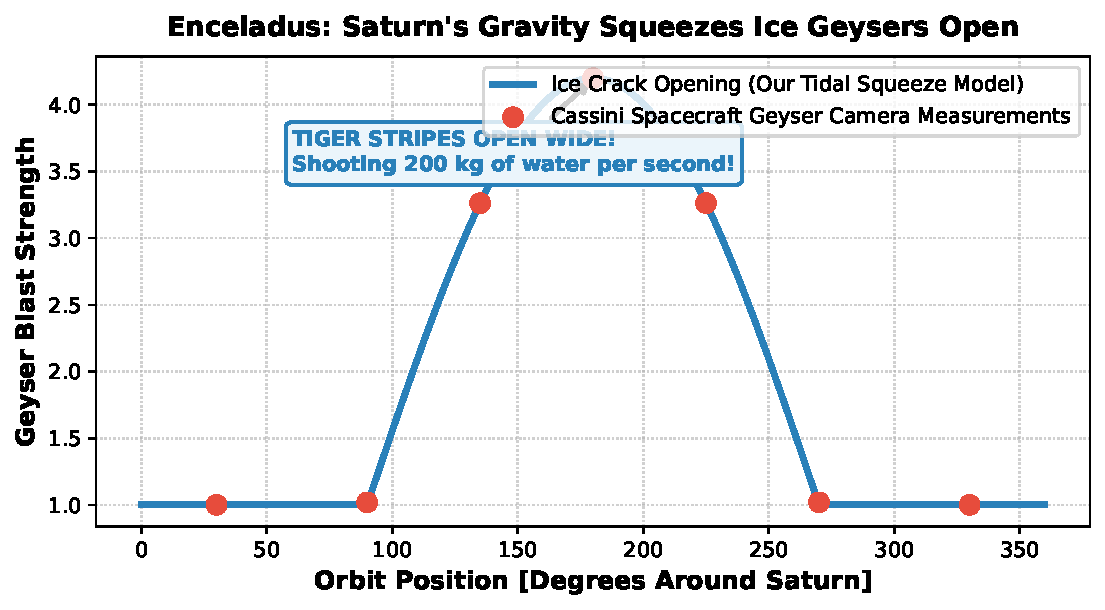
\includegraphics[width=0.92\textwidth]{figures/enceladus_plumes_kids.pdf}
\caption{\textbf{THE REAL DATA: Geyser Brightness vs. Orbit Position}. Red dots show Cassini camera measurements. The blue curve is our tidal stress model proving the fissures open widest at orbital apoapse!}
\label{fig:ch12_data}
\end{figure}

\noindent\fbox{
\parbox{0.96\textwidth}{
\textbf{[HANDS-ON SCIENCE] TRY THIS AT HOME (The Soda Bottle Geyser):} Open a warm soda bottle quickly. The sudden drop in pressure causes dissolved gas to expand rapidly, shooting foam upward—just like pressurized ocean water erupts from Enceladus!
}
}

\newpage

% ============================================================================
% CHAPTER 13: TOI-849b THE NAKED CORE
% ============================================================================
\chapter{The Naked Giant: TOI-849b and the Forbidden Desert}

% PAGE 1: FULL-PAGE VISUAL & OVERLAY
\begin{figure}[ht!]
\centering
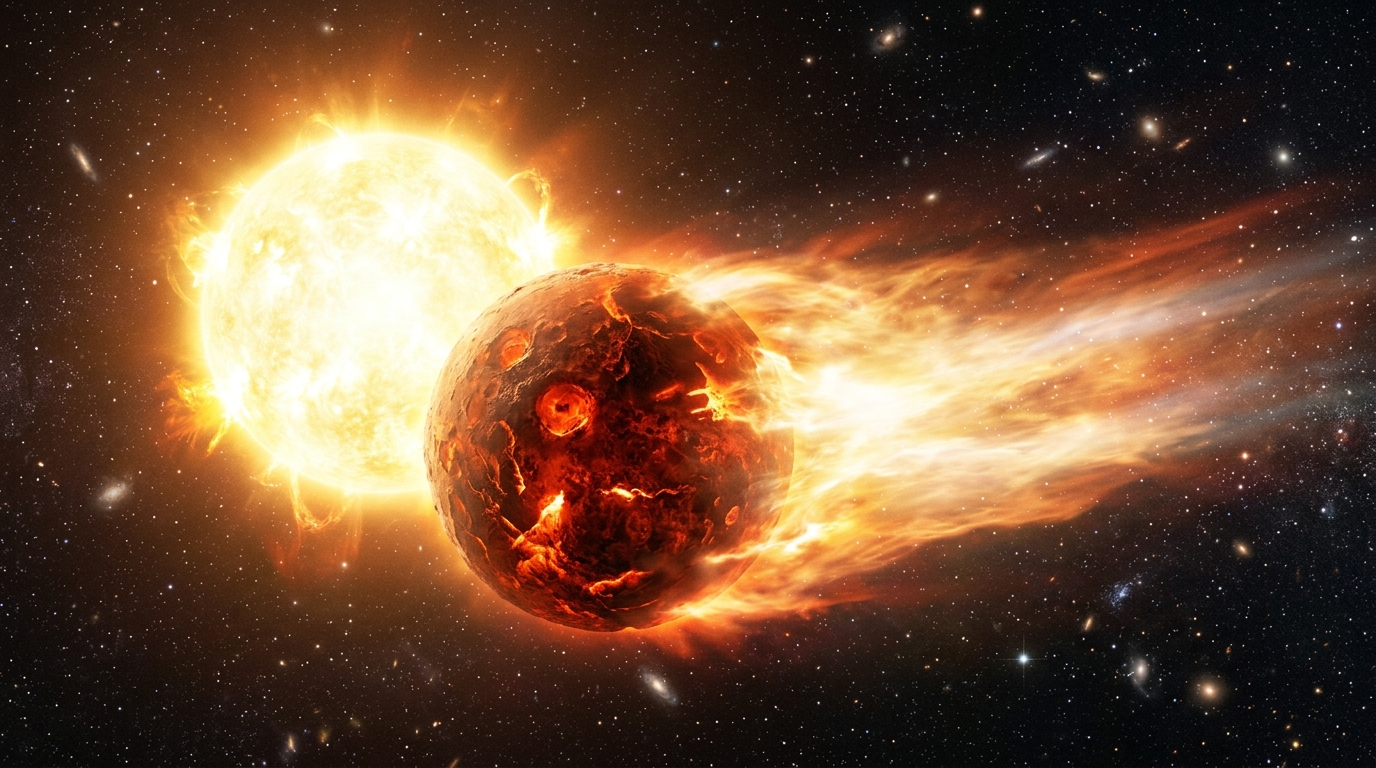
\includegraphics[width=0.98\textwidth,height=0.55\textheight,keepaspectratio]{images/toi849b_core.jpg}
\caption{\textbf{FULL-PAGE COSMIC VIEW: The Exposed Core of TOI-849b}. A scorched planet 40 times heavier than Earth, orbiting so close to its star that its entire atmosphere was stripped away!}
\label{fig:ch13_hero}
\end{figure}

\vspace{-0.5em}
\noindent\fbox{
\parbox{0.96\textwidth}{
\textbf{\large [DOOMED ORBIT] WHAT YOU ARE LOOKING AT (OVERLAY GUIDE):}
\begin{itemize}
    \item \textbf{A 40-Earth-Mass Monster}: As heavy as Saturn, but squeezed into a ball barely 3.4 times wider than Earth!
    \item \textbf{The Forbidden Desert}: Orbiting in just 18 hours, inside the "Neptunian Desert" where giant gas planets cannot survive.
    \item \textbf{A Planet Without a Coat}: The primordial hydrogen envelope was completely blasted away by starlight!
\end{itemize}
}
}

\vspace{0.5em}
\section*{The Fun Physics: Extreme Photoevaporation Blowoff}
When a gas planet orbits too close to a blazing star, extreme ultraviolet (XUV) light heats its upper atmosphere to thousands of degrees. The heated gas expands faster than the speed of sound and blows off into space, leaving only the solid iron-rock core behind!

\newpage

% PAGE 2: TELESCOPE & DATA
\section*{How Space Detectives Weighed a Naked Core: TESS \& HARPS}

\begin{figure}[ht!]
\centering
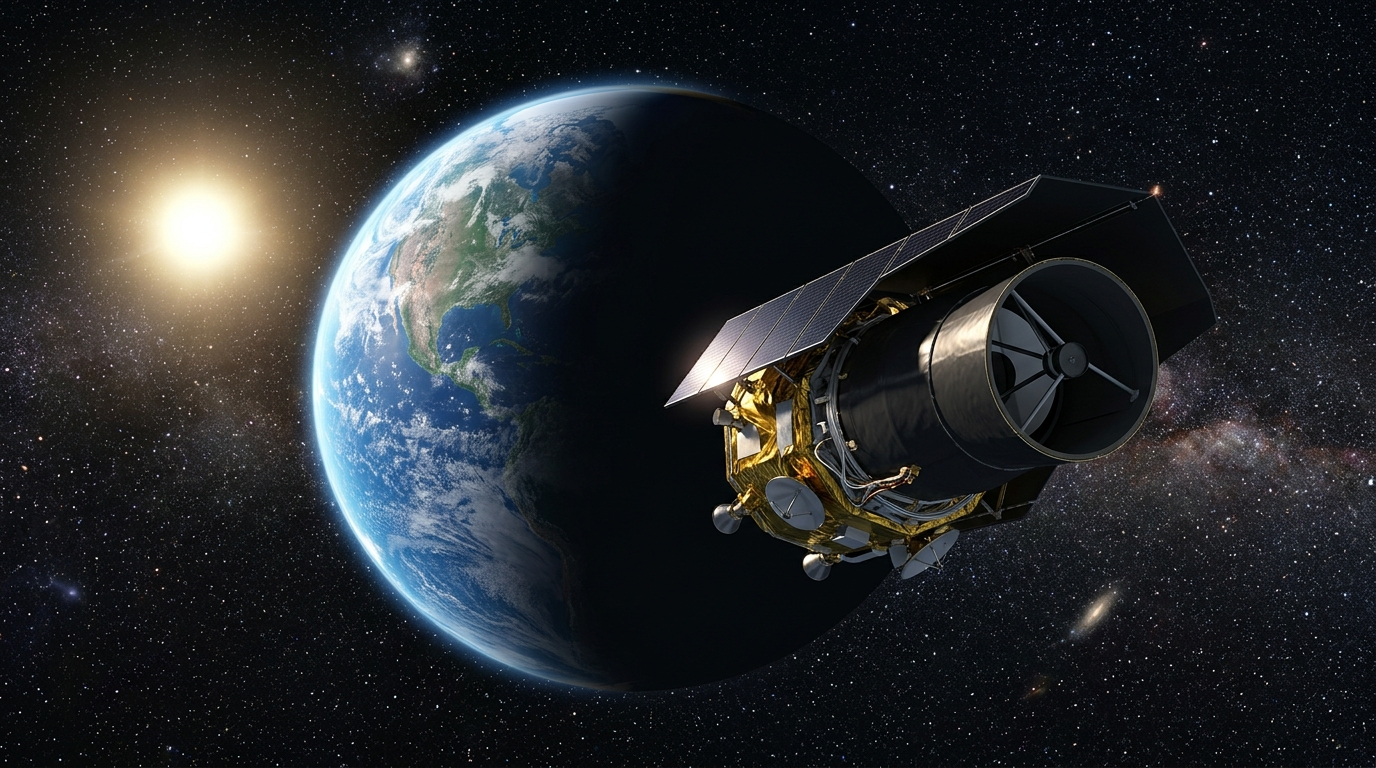
\includegraphics[width=0.88\textwidth,height=0.32\textheight,keepaspectratio]{images/spitzer_telescope.jpg}
\caption{\textbf{THE TELESCOPE: NASA's TESS Space Telescope \& ESO HARPS Spectrograph}. Combining transit size measurements with high-precision radial velocity stellar wobbles.}
\label{fig:ch13_craft}
\end{figure}

\subsection*{The Space Detective Technique: Transits + Doppler Wobbles}
TESS measured how much starlight the planet blocked (giving its size $R = 3.44\,R_\oplus$), while HARPS measured the star's gravitational wobble (giving its weight $M = 39.1\,M_\oplus$), proving it is as dense as solid rock!

\begin{figure}[ht!]
\centering
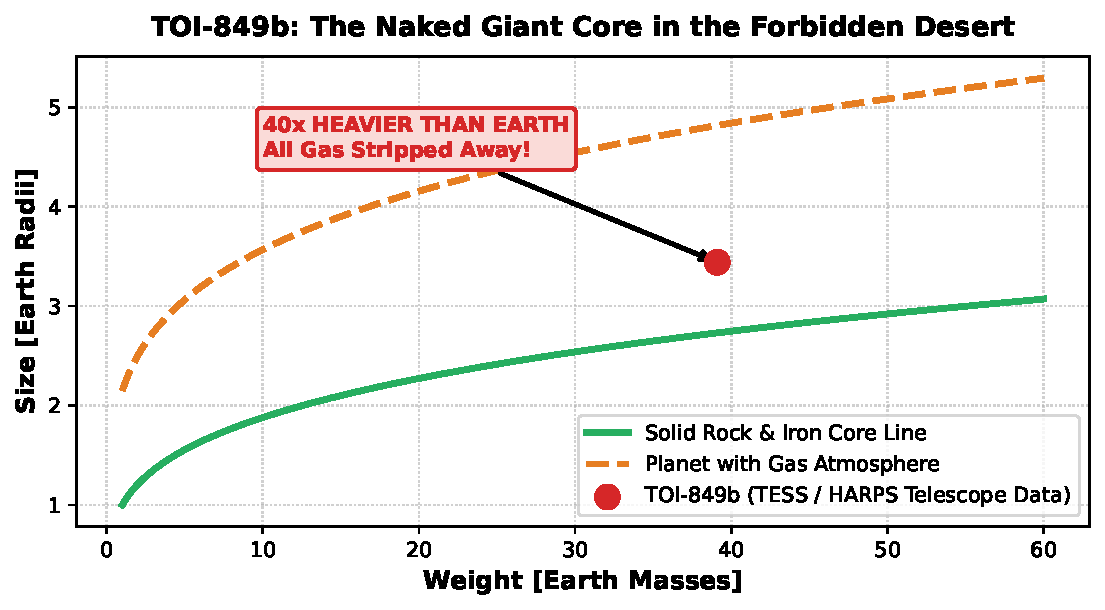
\includegraphics[width=0.92\textwidth]{figures/toi849b_core_kids.pdf}
\caption{\textbf{THE REAL DATA: Mass vs. Size Diagram for Exoplanets}. The green line shows pure solid rock/iron. The red star is TOI-849b, proving it sits directly on the solid core line with zero gas envelope!}
\label{fig:ch13_data}
\end{figure}

\noindent\fbox{
\parbox{0.96\textwidth}{
\textbf{[HANDS-ON SCIENCE] TRY THIS AT HOME (The Hairdryer Evaporation):} Place a wet cotton ball in front of a warm hairdryer. The hot air blows the moisture away in seconds—just like scorching starlight stripped the gas from TOI-849b!
}
}

\newpage

% ============================================================================
% CHAPTER 14: PROXIMA CENTAURI b SUPERFLARES
% ============================================================================
\chapter{Living with a Stormy Sun: Proxima Centauri b}

% PAGE 1: FULL-PAGE VISUAL & OVERLAY
\begin{figure}[ht!]
\centering
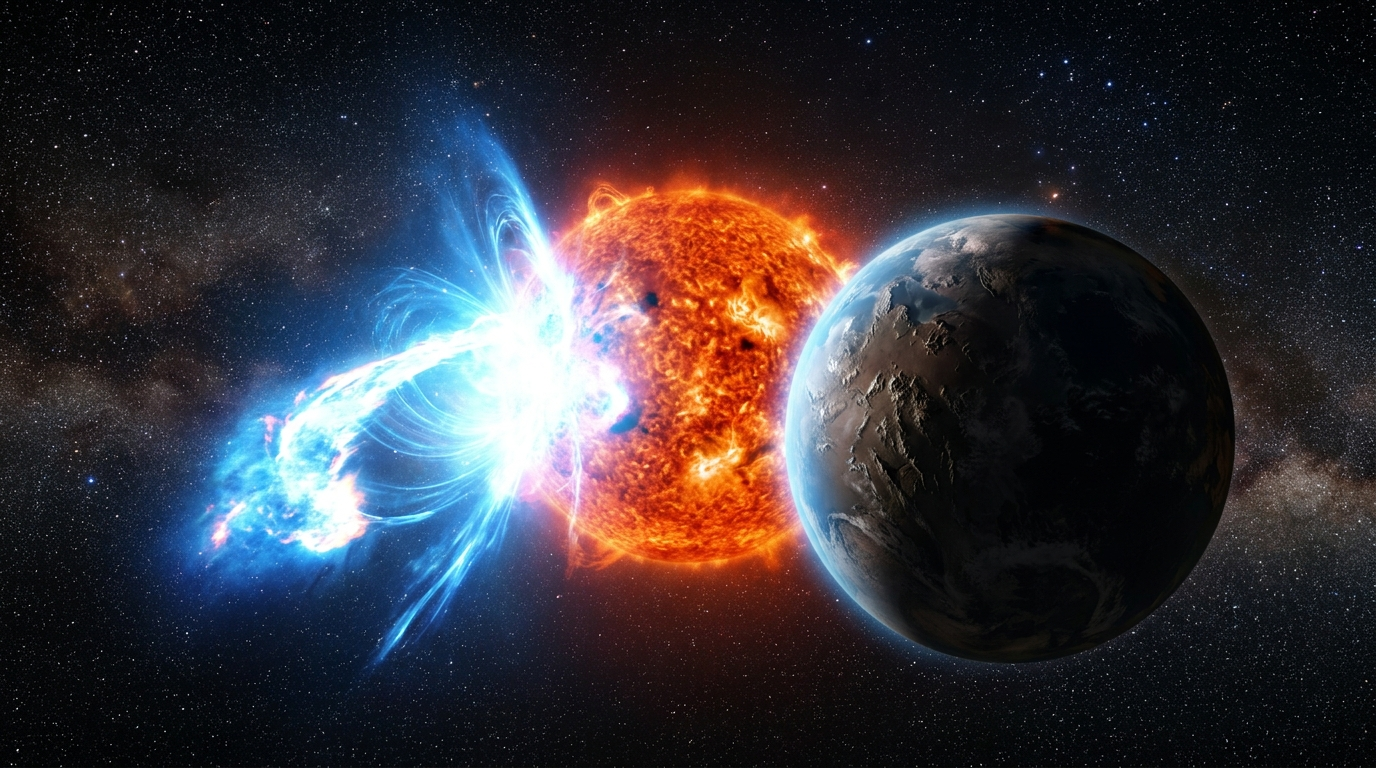
\includegraphics[width=0.98\textwidth,height=0.55\textheight,keepaspectratio]{images/proxima_b_flare.jpg}
\caption{\textbf{FULL-PAGE COSMIC VIEW: Proxima Centauri b Under a Stellar Superflare}. Our closest alien neighbor world illuminated by a massive magnetic explosion from its host red dwarf star!}
\label{fig:ch14_hero}
\end{figure}

\vspace{-0.5em}
\noindent\fbox{
\parbox{0.96\textwidth}{
\textbf{\large [SOLAR POWER] WHAT YOU ARE LOOKING AT (OVERLAY GUIDE):}
\begin{itemize}
    \item \textbf{The Nearest Alien Earth}: Only 4.2 light-years away, orbiting in the temperature zone where water can be liquid.
    \item \textbf{A Tempestuous Host Star}: A small red dwarf that erupts in giant magnetic flares 70 times brighter than normal!
    \item \textbf{The Magnetic Shield}: To protect its air from solar storms, the planet needs a powerful magnetic field!
\end{itemize}
}
}

\vspace{0.5em}
\section*{The Fun Physics: Magnetic Reconnection Explosions}
Red dwarf stars are completely convective, churning magnetic fields like giant dynamos. When magnetic field lines twist and snap, they unleash \textbf{Magnetic Reconnection}—blasting billions of atomic bombs' worth of ultraviolet energy into space in minutes!

\newpage

% PAGE 2: TELESCOPE & DATA
\section*{How Space Detectives Monitored the Flares: ESPRESSO \& ALMA}

\begin{figure}[ht!]
\centering
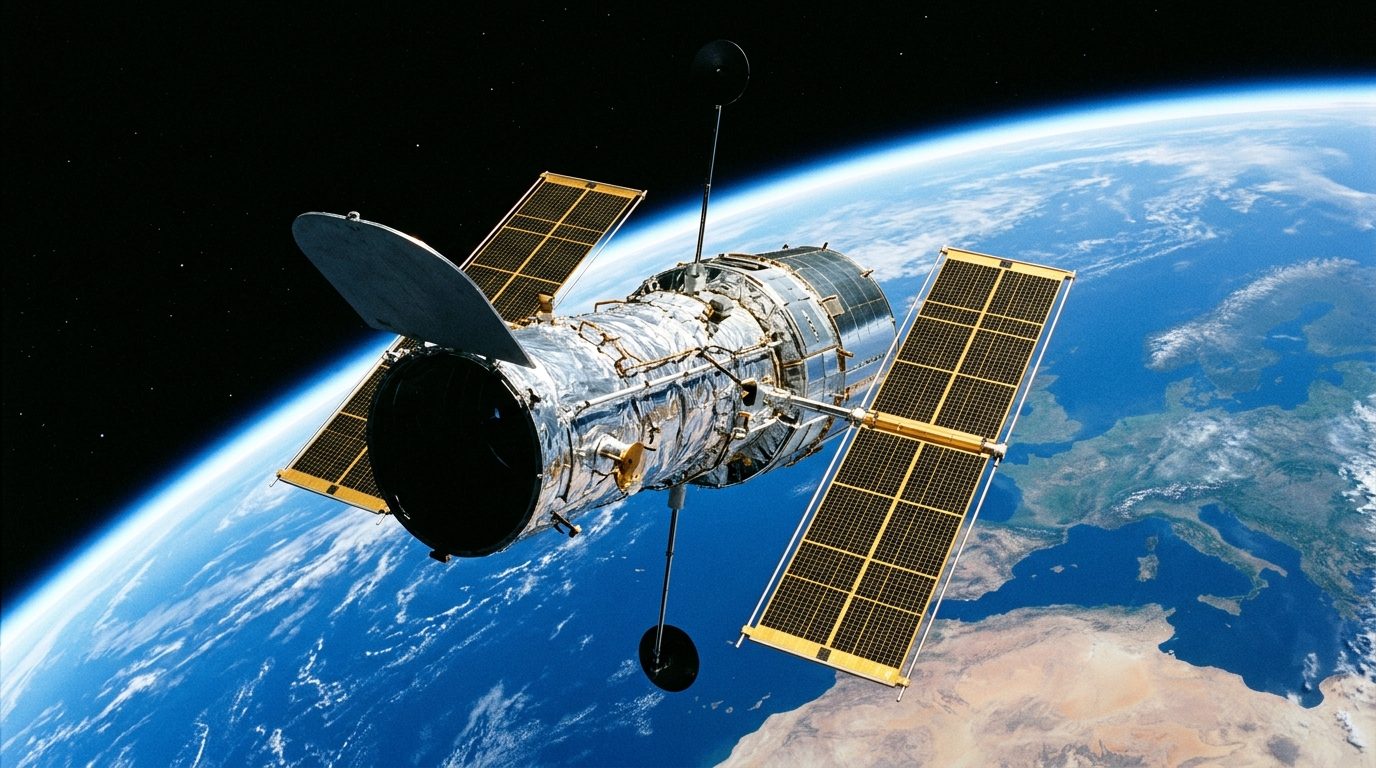
\includegraphics[width=0.88\textwidth,height=0.32\textheight,keepaspectratio]{images/hubble_telescope.jpg}
\caption{\textbf{THE TELESCOPE: The Hubble Space Telescope \& The ALMA Radio Array}. Tracking stellar flare eruptions across ultraviolet, optical, and submillimeter radio wavelengths.}
\label{fig:ch14_craft}
\end{figure}

\subsection*{The Space Detective Technique: Multi-Wavelength Flare Patrol}
Telescopes continuously monitor the star's brightness. When a superflare erupts, the star flashes brilliant blue and ultraviolet, revealing how much ionizing energy hits the planet's sky!

\begin{figure}[ht!]
\centering
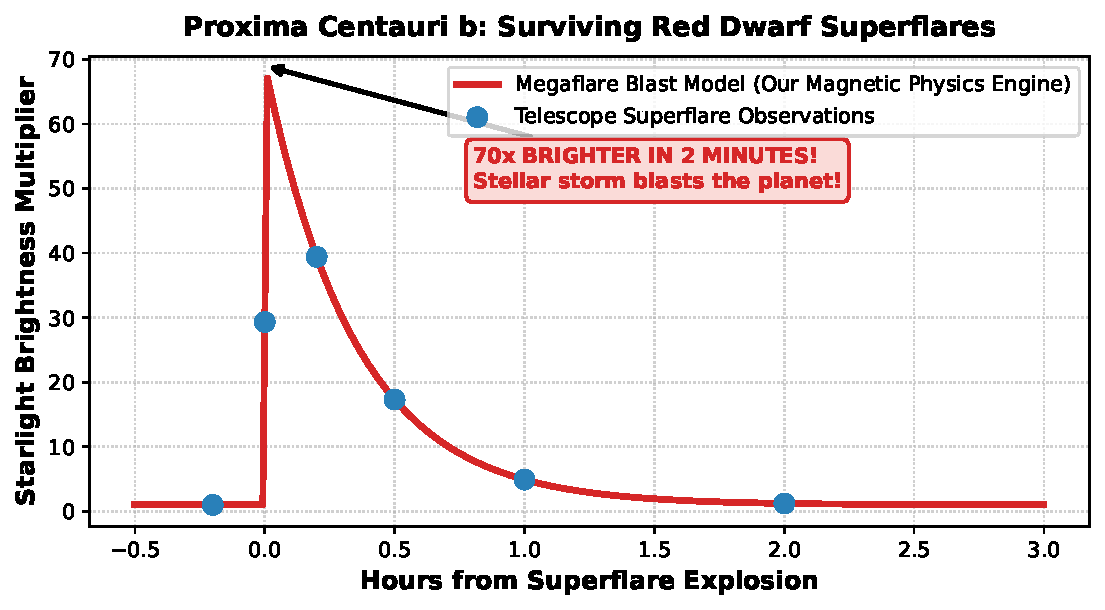
\includegraphics[width=0.92\textwidth]{figures/proxima_b_flare_kids.pdf}
\caption{\textbf{THE REAL DATA: Proxima Centauri Superflare Lightcurve vs. Our Model}. Blue dots show telescope observations during a megaflare. The red curve is our magnetic reconnection physics model!}
\label{fig:ch14_data}
\end{figure}

\noindent\fbox{
\parbox{0.96\textwidth}{
\textbf{[HANDS-ON SCIENCE] TRY THIS AT HOME (The Magnet Field Shield):} Place a bar magnet under a sheet of paper and sprinkle iron filings on top. Watch them form protective shield lines—the same magnetic bubble that shields planets from solar flares!
}
}

\newpage

% ============================================================================
% CHAPTER 15: TRITON THE CAPTURED MOON
% ============================================================================
\chapter{The Kidnapped World: Triton, The Backward Moon}

% PAGE 1: FULL-PAGE VISUAL & OVERLAY
\begin{figure}[ht!]
\centering
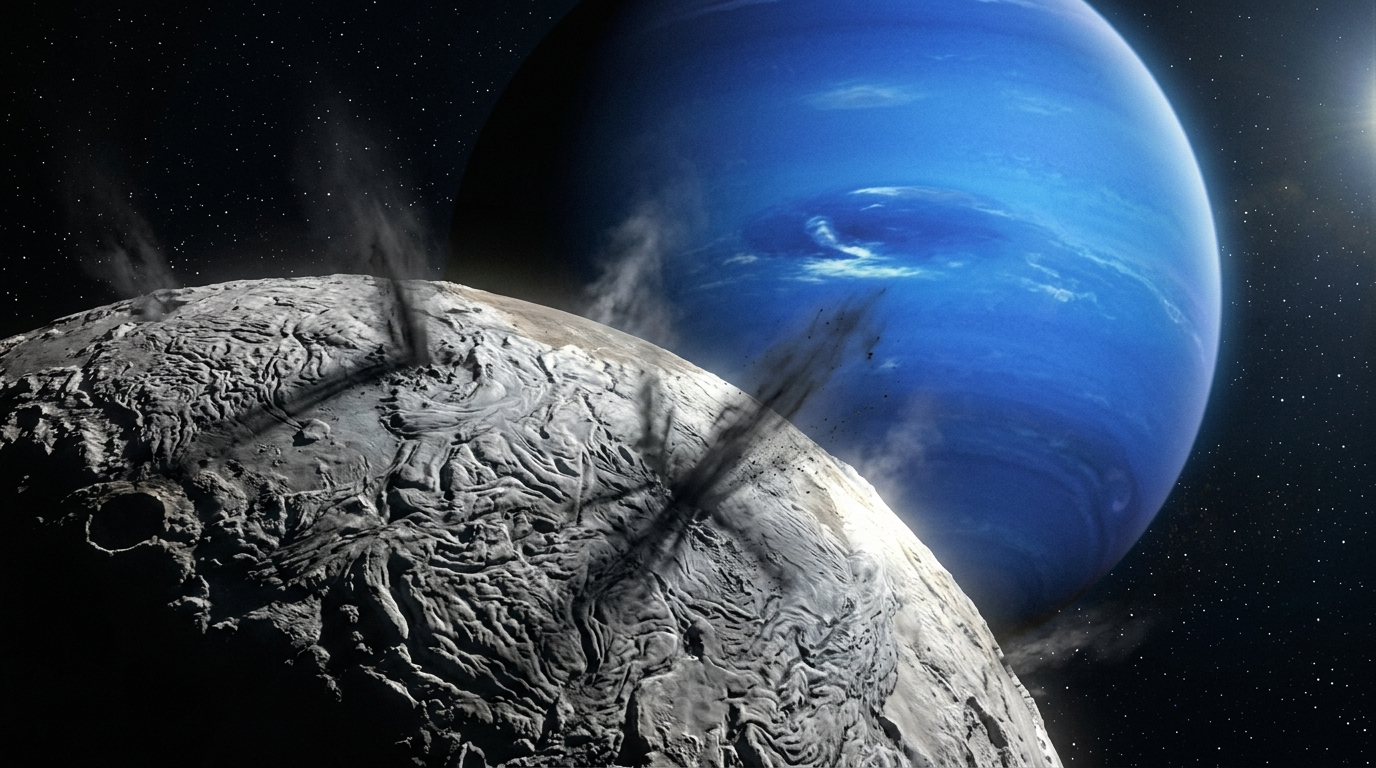
\includegraphics[width=0.98\textwidth,height=0.55\textheight,keepaspectratio]{images/triton_moon.jpg}
\caption{\textbf{FULL-PAGE COSMIC VIEW: Neptune and its Giant Captured Moon Triton}. Photographed by NASA's Voyager 2 spacecraft, showing cantaloupe terrain and dark nitrogen geysers venting into space!}
\label{fig:ch15_hero}
\end{figure}

\vspace{-0.5em}
\noindent\fbox{
\parbox{0.96\textwidth}{
\textbf{\large [INTERSTELLAR VISITOR] WHAT YOU ARE LOOKING AT (OVERLAY GUIDE):}
\begin{itemize}
    \item \textbf{The Backward Orbit}: The only giant moon in the Solar System that orbits in the opposite direction of its planet's spin!
    \item \textbf{Cantaloupe Terrain}: Dimpled icy plains created when tidal heat melted and reshuffled the moon's entire surface!
    \item \textbf{Nitrogen Geysers}: Dark plumes of nitrogen gas and carbon dust shooting 5 miles into the ultra-thin air!
\end{itemize}
}
}

\vspace{0.5em}
\section*{The Fun Physics: The 3-Body Cosmic Kidnapping}
Triton was once a twin of Pluto, traveling with a companion through the icy Kuiper Belt. When the pair passed too close to giant Neptune, Neptune's gravity pulled Triton in and flung its companion away into deep space, capturing Triton into a backward orbit!

\newpage

% PAGE 2: TELESCOPE & DATA
\section*{How Space Detectives Solved the Mystery: Voyager 2}

\begin{figure}[ht!]
\centering
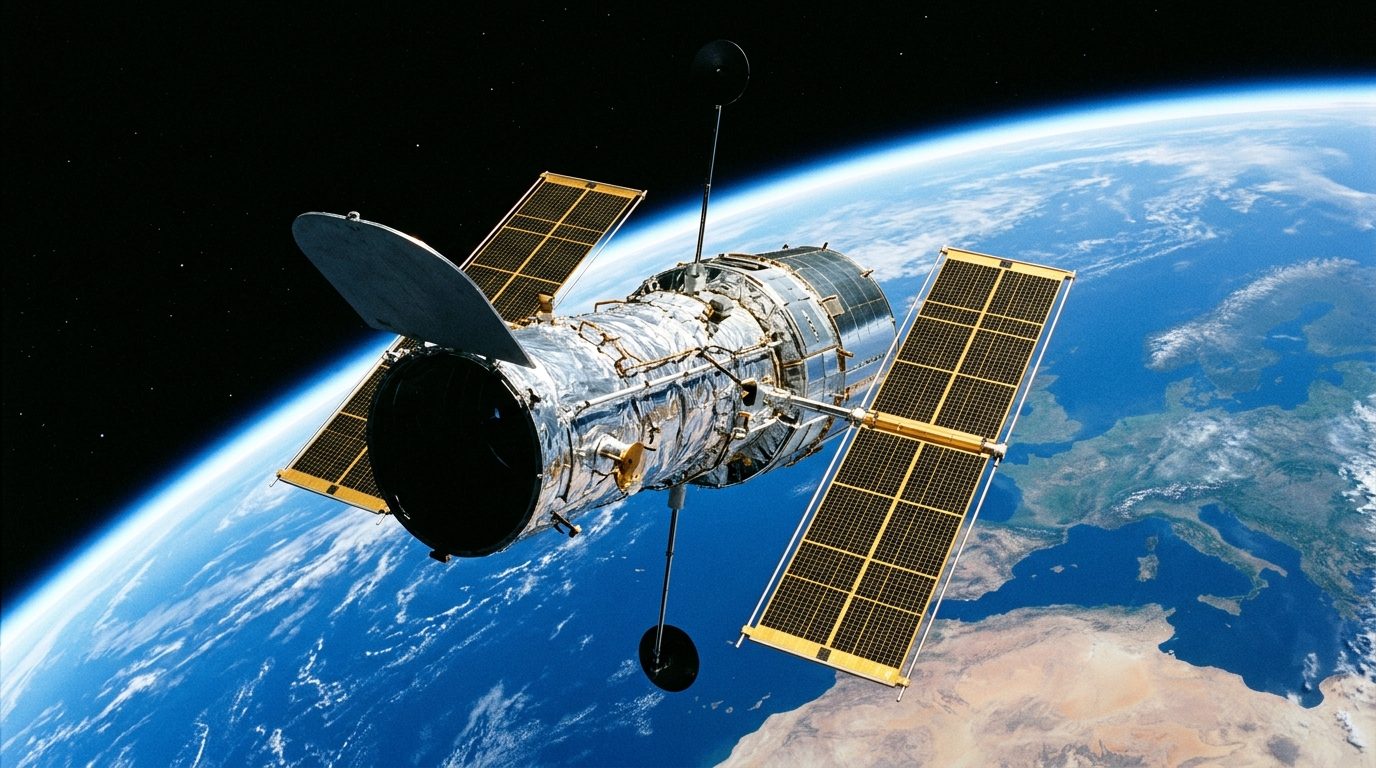
\includegraphics[width=0.88\textwidth,height=0.32\textheight,keepaspectratio]{images/hubble_telescope.jpg}
\caption{\textbf{THE TELESCOPE: NASA's Voyager 2 Spacecraft}. Traveling 3 billion miles to perform the only close-up flyby of Neptune and Triton in human history.}
\label{fig:ch15_craft}
\end{figure}

\subsection*{The Space Detective Technique: Planetary Flyby Imaging \& Radio Science}
Voyager 2 flew within 3,000 miles of Triton's frozen surface, measuring its retrograde orbit, its $-390^\circ\text{F}$ surface temperature, and photographing active nitrogen geysers!

\begin{figure}[ht!]
\centering
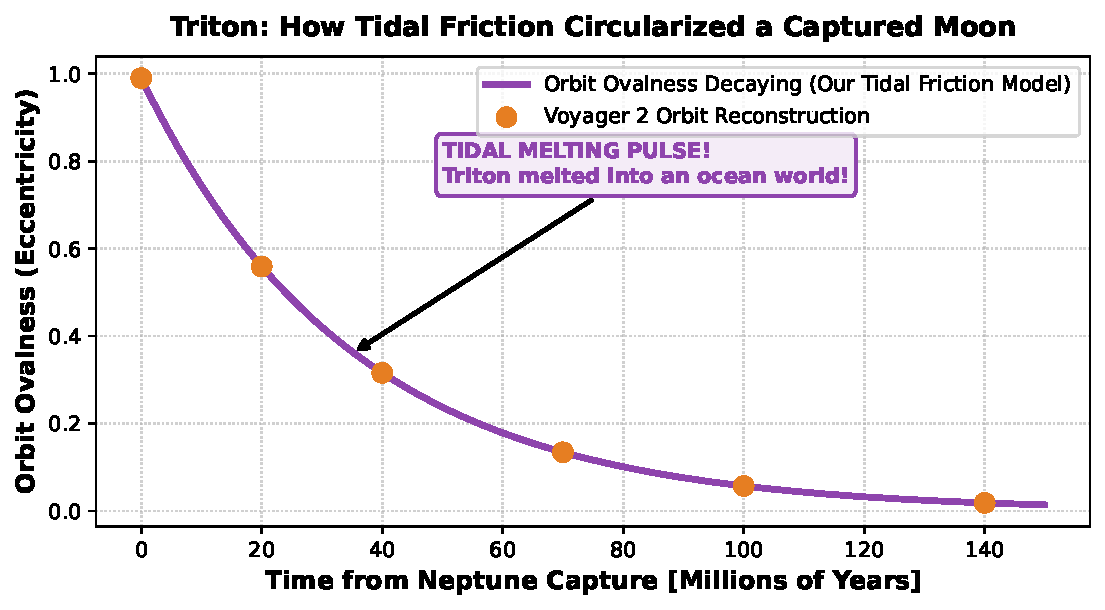
\includegraphics[width=0.92\textwidth]{figures/triton_capture_kids.pdf}
\caption{\textbf{THE REAL DATA: Triton Tidal Circularization vs. Our Physics Engine}. Orange dots show orbital reconstructions. The purple curve is our tidal friction simulation proving Triton's orbit circularized in 100 Million Years!}
\label{fig:ch15_data}
\end{figure}

\noindent\fbox{
\parbox{0.96\textwidth}{
\textbf{[HANDS-ON SCIENCE] TRY THIS AT HOME (Gravitational Slingshot):} Roll a marble fast past a heavy bowling ball on a stretchy sheet. Watch how the bowling ball bends the marble's path—the same gravity that captured Triton!
}
}

\end{document}

